\documentclass[xcolor=dvipsnames]{beamer}

\geometry{paperwidth=140mm,paperheight=105mm}

\usepackage[utf8x]{inputenc}
\usepackage{amsmath,amsfonts,amssymb}
\usecolortheme{default}
\usepackage{graphicx}
\usepackage{tikz}
\usepackage{caption}
\usepackage{nicefrac}
\usepackage{mathabx}
\usepackage{hyperref}
%\usepackage{wrapfig}
% %\usepackage{cutwin}

\definecolor{DarkBlue}{HTML}{002e77}

\newcommand{\averx}{\langle x \rangle}
\newcommand{\Raverx}{\averx_\mathrm{ren}}

\usetheme{Boadilla}
\usecolortheme[named=DarkBlue]{structure}
\useinnertheme{rounded}

\usefonttheme{professionalfonts}
\setbeamertemplate{navigation symbols}{}
\setbeamertemplate{enumerate items}[square]

\usepackage{algorithm}
\usepackage{algorithmicx}
\usepackage{algpseudocode}

\makeatletter
\renewcommand{\ALG@beginalgorithmic}{\small}
\makeatother

\usepackage{sourcecodepro}
\usepackage{listings}
\definecolor{mygreen}{rgb}{0,0.6,0}
\definecolor{mygray}{rgb}{0.5,0.5,0.5}
\definecolor{mymauve}{rgb}{0.58,0,0.82}
% \PassOptionsToPackage{svgnames}{xcolor}

\lstset{ %
  backgroundcolor=\color{white},   % choose the background color; you must add \usepackage{color} or \usepackage{xcolor}; should come as last argument
  basicstyle=\footnotesize\ttfamily, % the size of the fonts that are used for the code
  breakatwhitespace=false,         % sets if automatic breaks should only happen at whitespace
  breaklines=true,                 % sets automatic line breaking
  captionpos=b,                    % sets the caption-position to bottom
  commentstyle=\color{mygreen},    % comment style
  deletekeywords={...},            % if you want to delete keywords from the given language
  escapeinside={\%*}{*)},          % if you want to add LaTeX within your code
  extendedchars=false,              % lets you use non-ASCII characters; for 8-bits encodings only, does not work with UTF-8
  frame=single,	                   % adds a frame around the code
  keepspaces=true,                 % keeps spaces in text, useful for keeping indentation of code (possibly needs columns=flexible)
  keywordstyle=\color{blue},       % keyword style
  language=C,                      % the language of the code
  morekeywords={*,...},            % if you want to add more keywords to the set
  numbers=none,                    % where to put the line-numbers; possible values are (none, left, right)
  numbersep=5pt,                   % how far the line-numbers are from the code
  numberstyle=\tiny\color{mygray}, % the style that is used for the line-numbers
  rulecolor=\color{black},         % if not set, the frame-color may be changed on line-breaks within not-black text (e.g. comments (green here))
  showspaces=false,                % show spaces everywhere adding particular underscores; it overrides 'showstringspaces'
  showstringspaces=false,          % underline spaces within strings only
  showtabs=false,                  % show tabs within strings adding particular underscores
  stepnumber=1,                    % the step between two line-numbers. If it's 1, each line will be numbered
  stringstyle=\color{mymauve},     % string literal style
  tabsize=2,	                   % sets default tabsize to 2 spaces
  moredelim=**[is][\color{red}]{!@}{!@},
  %title=\lstname                   % show the filename of files included with \lstinputlisting; also try caption instead of title
}

\renewcommand{\UrlFont}{\small}

\newcounter{lecturecounter}
\setcounter{lecturecounter}{1}

\author[B. Kostrzewa]{Bartosz Kostrzewa, Ferenc Pittler, Martin Ueding, Carsten Urbach}
\title{C-Kurs Physik, 2017}
\institute[HISKP]{HISKP, Rheinische Friedrich-Wilhelms-Universität Bonn}
% \titlegraphic{\roundbox{\includegraphics[height=2cm]{UniBonn_CRC110_ETMC_INFN}}}
\date[April 2017]{April 2017}

\begin{document}

% \frame{}
\begin{frame}
 \titlepage
\end{frame}

\begin{frame}{Administrativa}
  \begin{itemize}
  \item{Vorlesung 03.04-13.04, 10-12 Uhr, \textbf{PI HS1}}
  \begin{itemize}
    \item{06.04: \textbf{HS HISKP} }
  \end{itemize}
  \vspace{0.2cm}
  \item{Bartosz Kostrzewa, bartosz\_kostrzewa@fastmail.com, Raum 3.009 HISKP}
  \begin{itemize}
    \item{Sprechzeiten: Täglich 17:00-17:45 Uhr}
  \end{itemize}
  \vspace{0.2cm}
  \item{Tutoren}
  \begin{itemize}
    \item{Martin~Ueding, Simon~Schlepphorst, 
         \\Ferenc~Pittler, Marcel~Nitsch, Florian~Tauber} 
  \end{itemize}
  \vspace{0.2cm}
  \item{Tutorien finden statt: täglich 13:00-17:00}
  \begin{itemize}
    \item{Astro CIP Pool (Raum 0.007) [AifA, Auf dem Hügel 71]}
    \item{HISKP SR1 [HISKP, Nußallee 14-16]}
    \begin{itemize}
      \item{\textbf{ $\mathbf{18}$ Personen $\rightarrow$ Astro, $\quad\mathbf{N-18}$ $\rightarrow$ SR1} }
    \end{itemize}
  \end{itemize}
  \vspace{0.2cm}
  \item{Das Skript dient als Referenz und sollte zumindest während der Tutorien befragt werden!}
  \vspace{0.2cm}
  \item{Fundamentale Ungleichung der Programmierung (FUP!): \\ \textbf{Praxis $\mathbf{\gg}$ Vorlesungen} $\rightarrow$ besuchen Sie die Übungen, sonst bringt die Vorlesung nichts!}
  \item{Folien, Übungszettel, Beispielprogramme: \textcolor{blue}{\url{http://goo.gl/xhJN08}}}
  \end{itemize}
\end{frame}

\begin{frame}{Lernziele}
\begin{itemize}
  \item{Algorithmen verstehen und entwickeln}
  \item{Algorithmen in Quelltext übertragen}
  \vspace{0.3cm}
  \item{Erstes Kennenlernen der sogennanten \emph{imperativen} Programmierung}
  \item{Kennenlernen der Daten- und Kontrollstrukturen von C99}
  \vspace{0.3cm}
  \item{Praktischer Einsatz des C-Compilers zur Übersetzung des Quelltextes in ausführbaren Maschinencode}
  \item{Erstellen eigener C-Programme in den Tutorien}
  \begin{itemize}
    \item{einfache Beispielprogramme $\rightarrow$ kompliziertere Programme aus merheren Quelltextdateien}
    \item{Verwendung externer Bilbiotheken}
  \end{itemize}
  \vspace{0.3cm}
  \item{Vorbereitung auf \emph{physik441: Computerphysik} (SoSe 2017), \emph{physics760: Computational Physics} (WiSe 2017/2018), etwaige Bachelor- und Masterarbeiten}
\end{itemize} 
\end{frame}

\begin{frame}{Anwendung: Plasmaphysik / Fusion}
  \centering
  Wellenstein 7-x Stellerator\\ \vspace{0.2cm}
  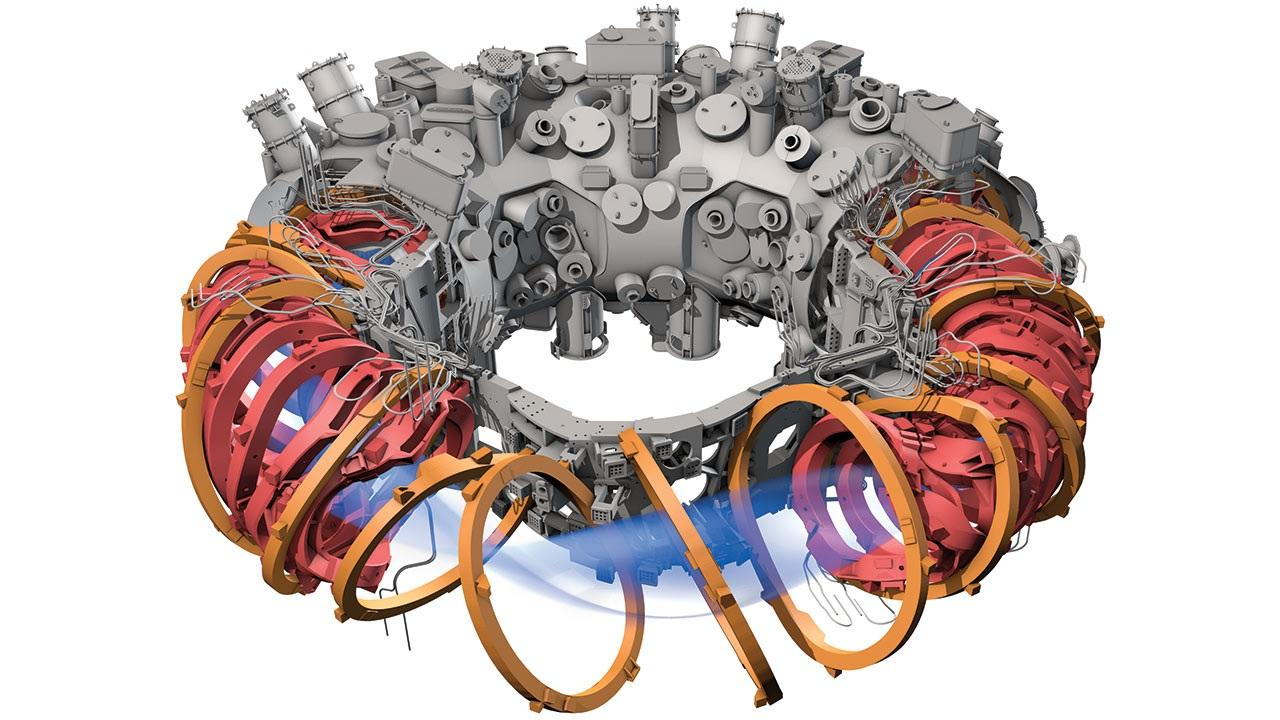
\includegraphics[width=0.9\textwidth]{graphics/stellerator.jpg}\\
  {\small Quelle: \url{http://www.sciencemag.org/news/2015/10/bizarre-reactor-might-save-nuclear-fusion} }
\end{frame}

\begin{frame}{Anwendung: Kosmologie / Astrophysik}
  \centering
  Simulation der Galaxie M74 über 13 Milliarden Jahre\\ \vspace{0.2cm}
  
\includegraphics[width=0.9\textwidth]{graphics/m74_simulation.png}\\
  {\small Quelle: \url{http://www.hpc-ch.org/first-realistic-simulation-of-the-formation-of-the-milky-way-computed-at-cscs/} }  
\end{frame}

\begin{frame}{Anwendung: Hochenergiephysik - LHC}
  \centering
  Kollision im ATLAS-Experiment\\ \vspace{0.2cm}
  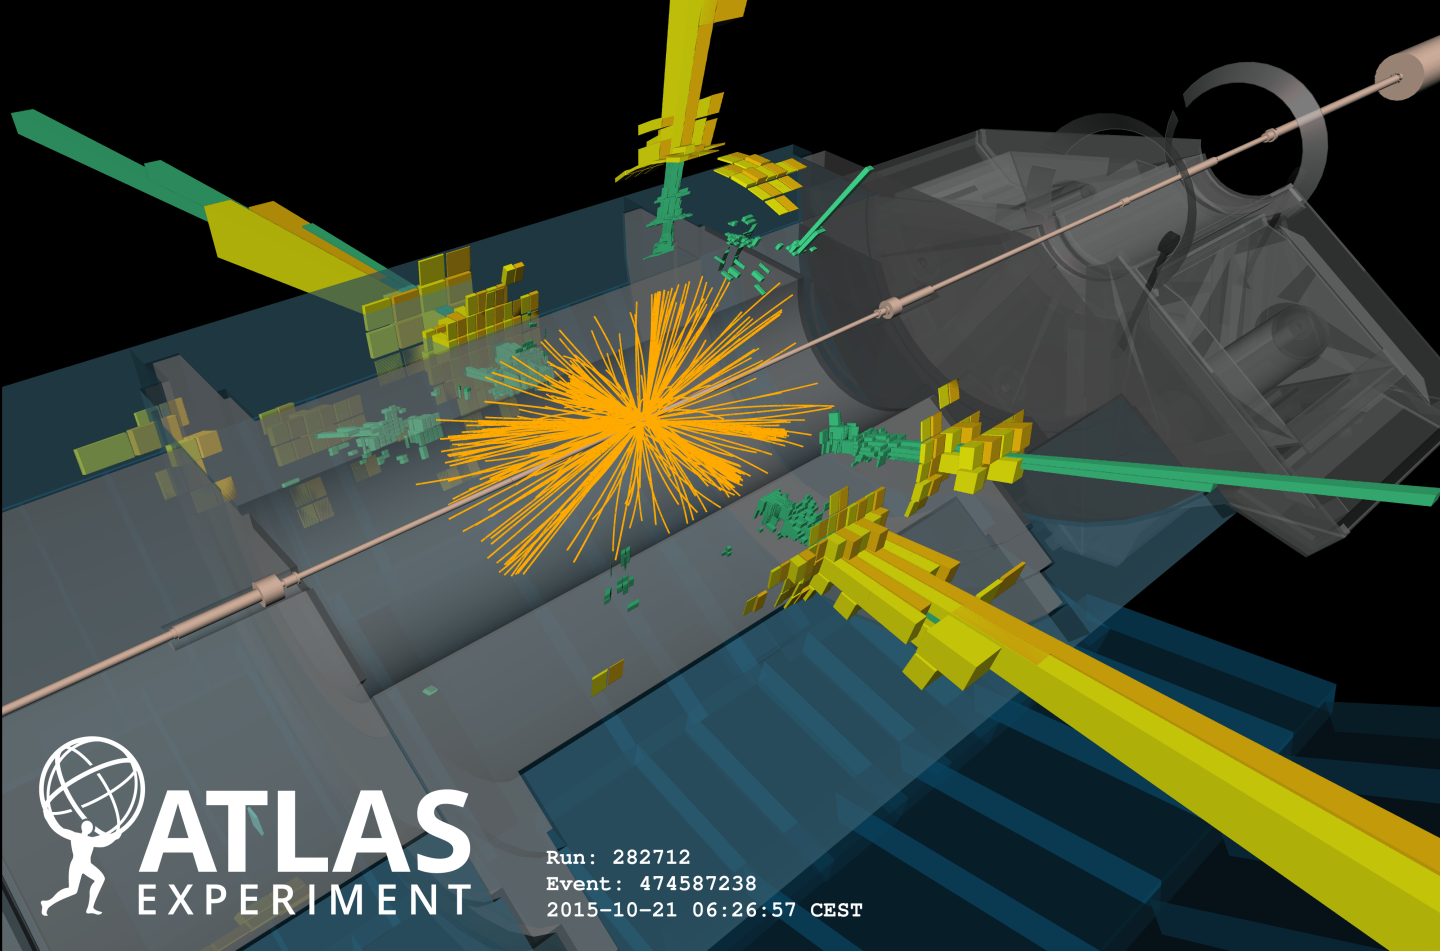
\includegraphics[width=0.9\textwidth]{graphics/atlas_event.png}\\
  {\small Quelle: \url{ https://cds.cern.ch/record/2113241 } }
\end{frame}

\begin{frame}{Anwendung: Hochenergiephysik / Gitter-QCD}
  \centering
  Simulation der Quantenchromodynamik auf Hochgeschwindigkeitsrechnern\\ \vspace{0.2cm}
  \begin{columns}
  \column{0.49\textwidth}
    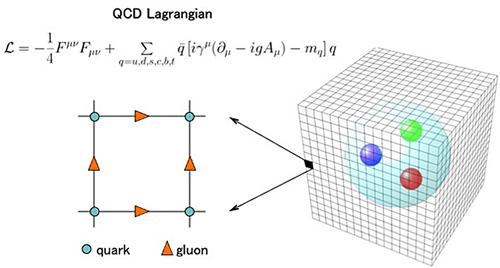
\includegraphics[width=0.8\textwidth]{graphics/LQCD2.jpg} \\
  \column{0.49\textwidth}
    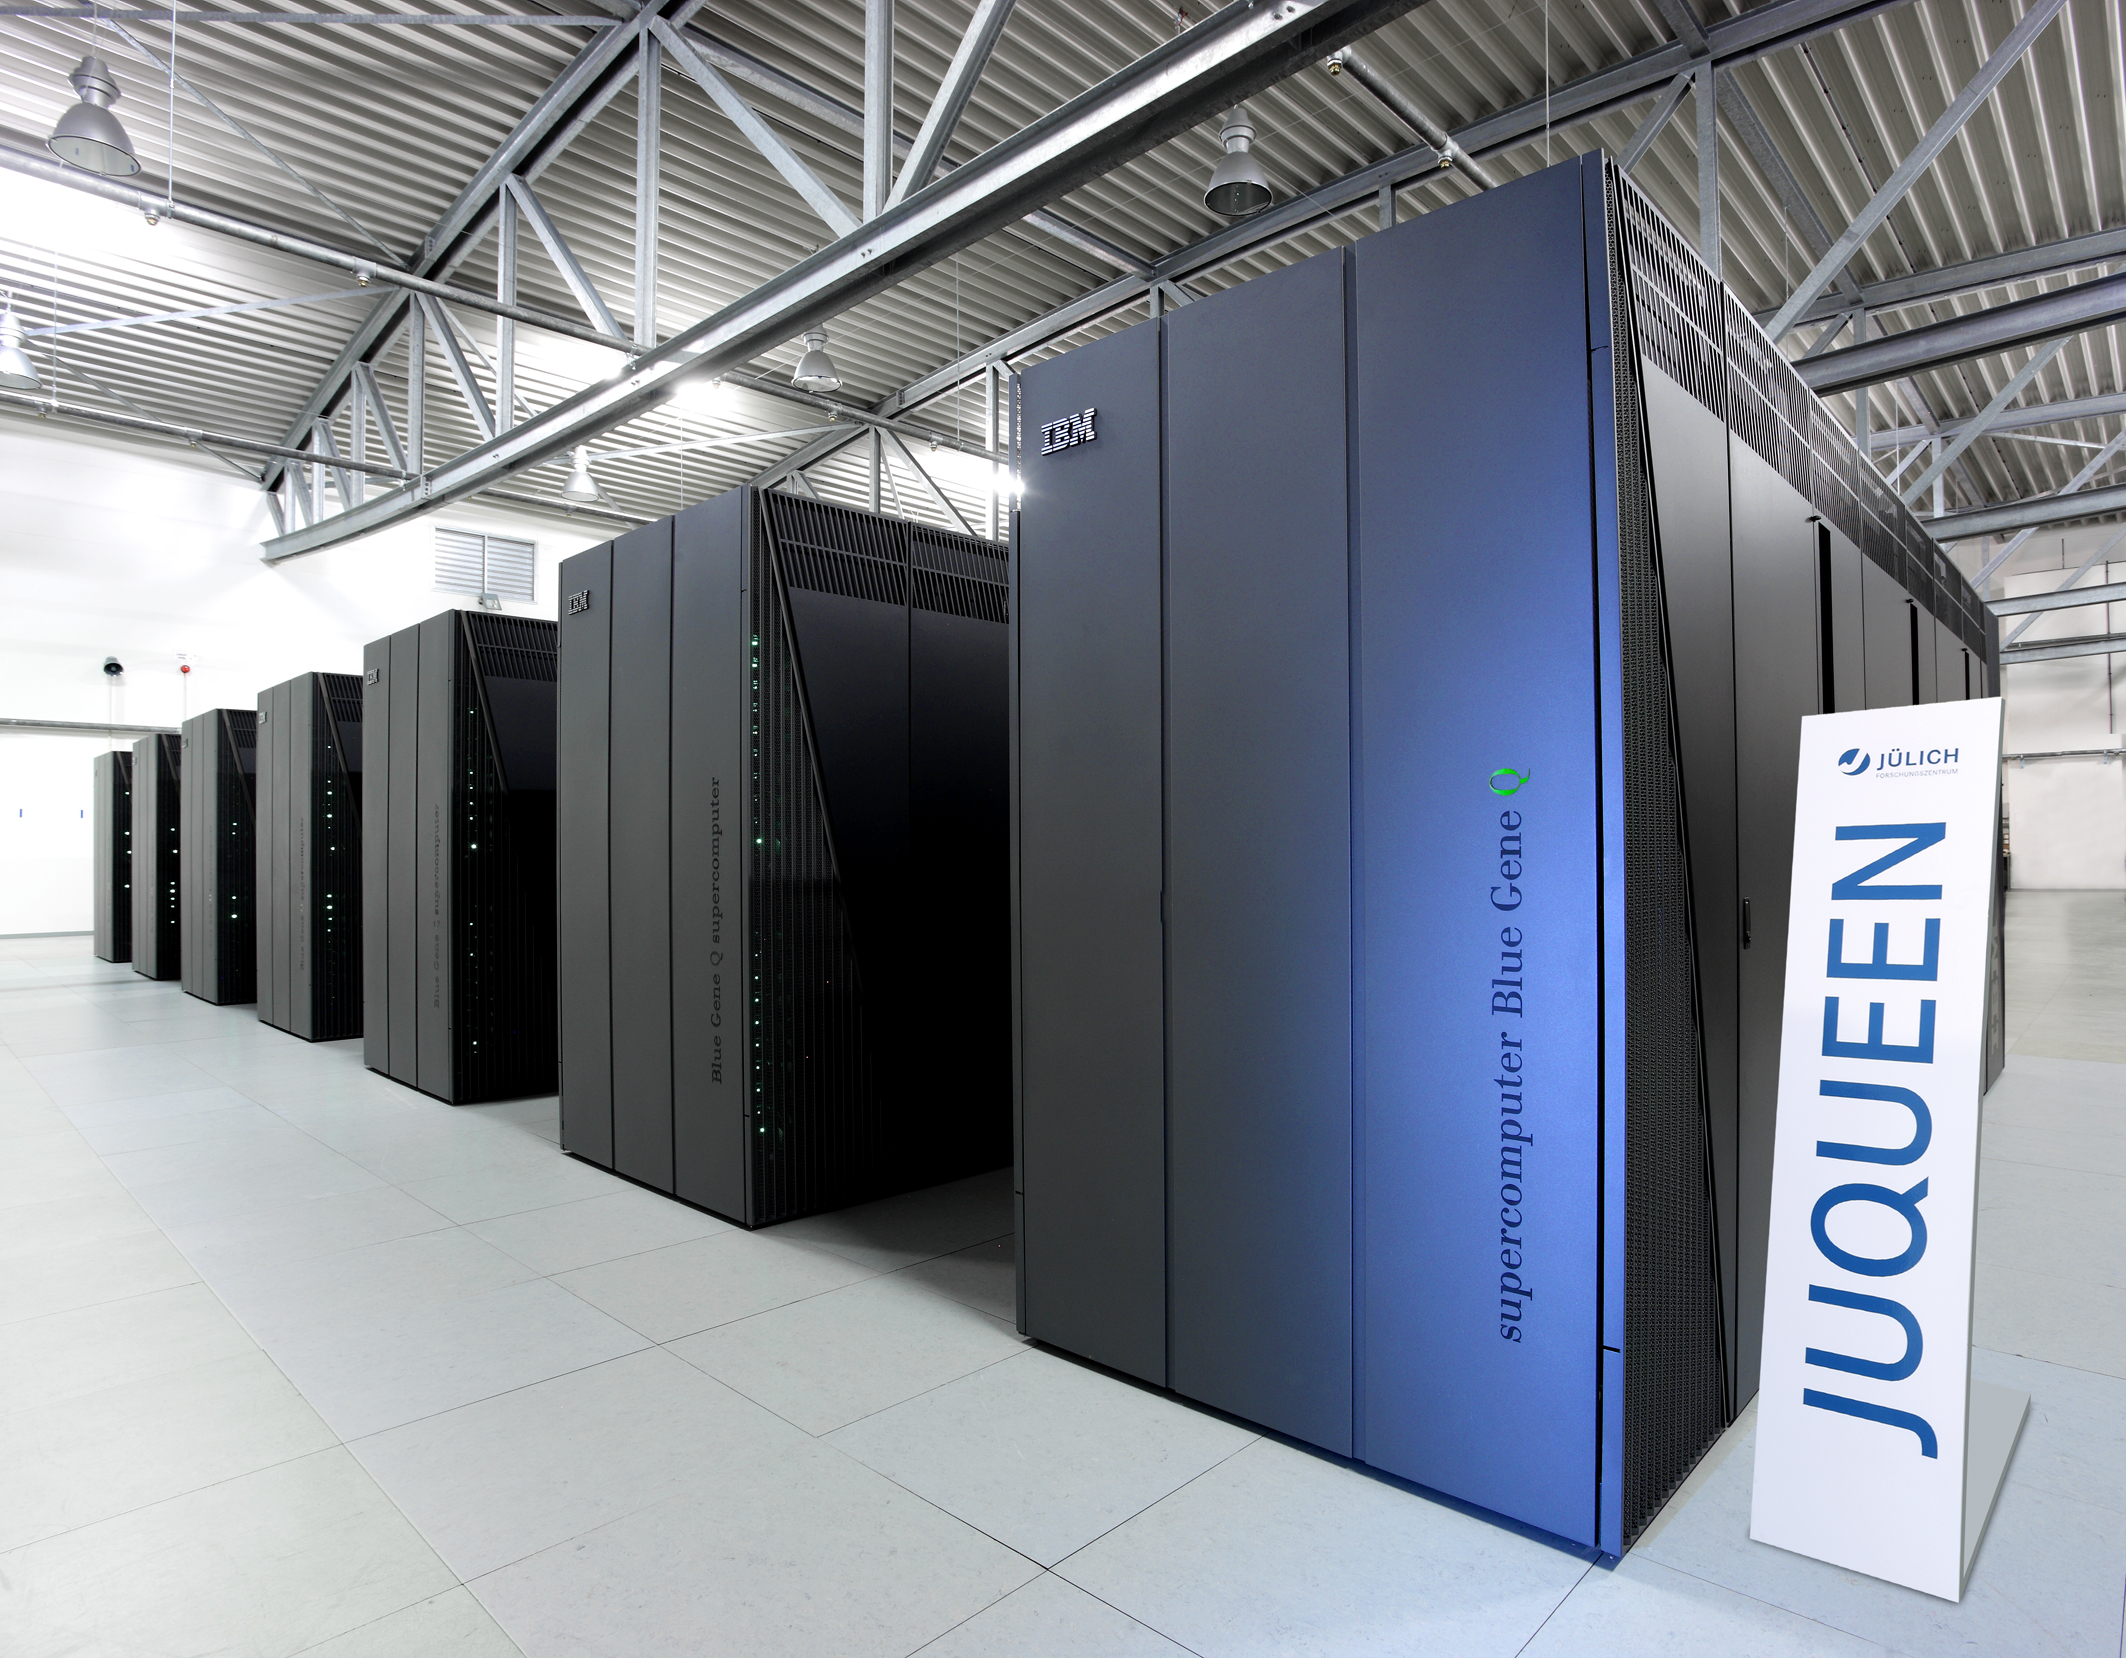
\includegraphics[width=0.8\textwidth]{graphics/juqueen.jpg} \\
  \end{columns}
  \vspace{0.3cm}
  {\small Quellen: \url{http://lpc-clermont.in2p3.fr/IMG/theorie/LQCD2.jpg} \\
                   \url{http://www.fz-juelich.de/ias/jsc/EN/Expertise/Supercomputers/JUQUEEN/JUQUEEN_node.html} }
\end{frame}

\begin{frame}{Anwendung: Biophysik / Biochemie - Molekulardynamik}
  \centering
  Simulation des NMDA Proteins und Rezeptors im menschlichen Gehirn\\ \vspace{0.2cm}
  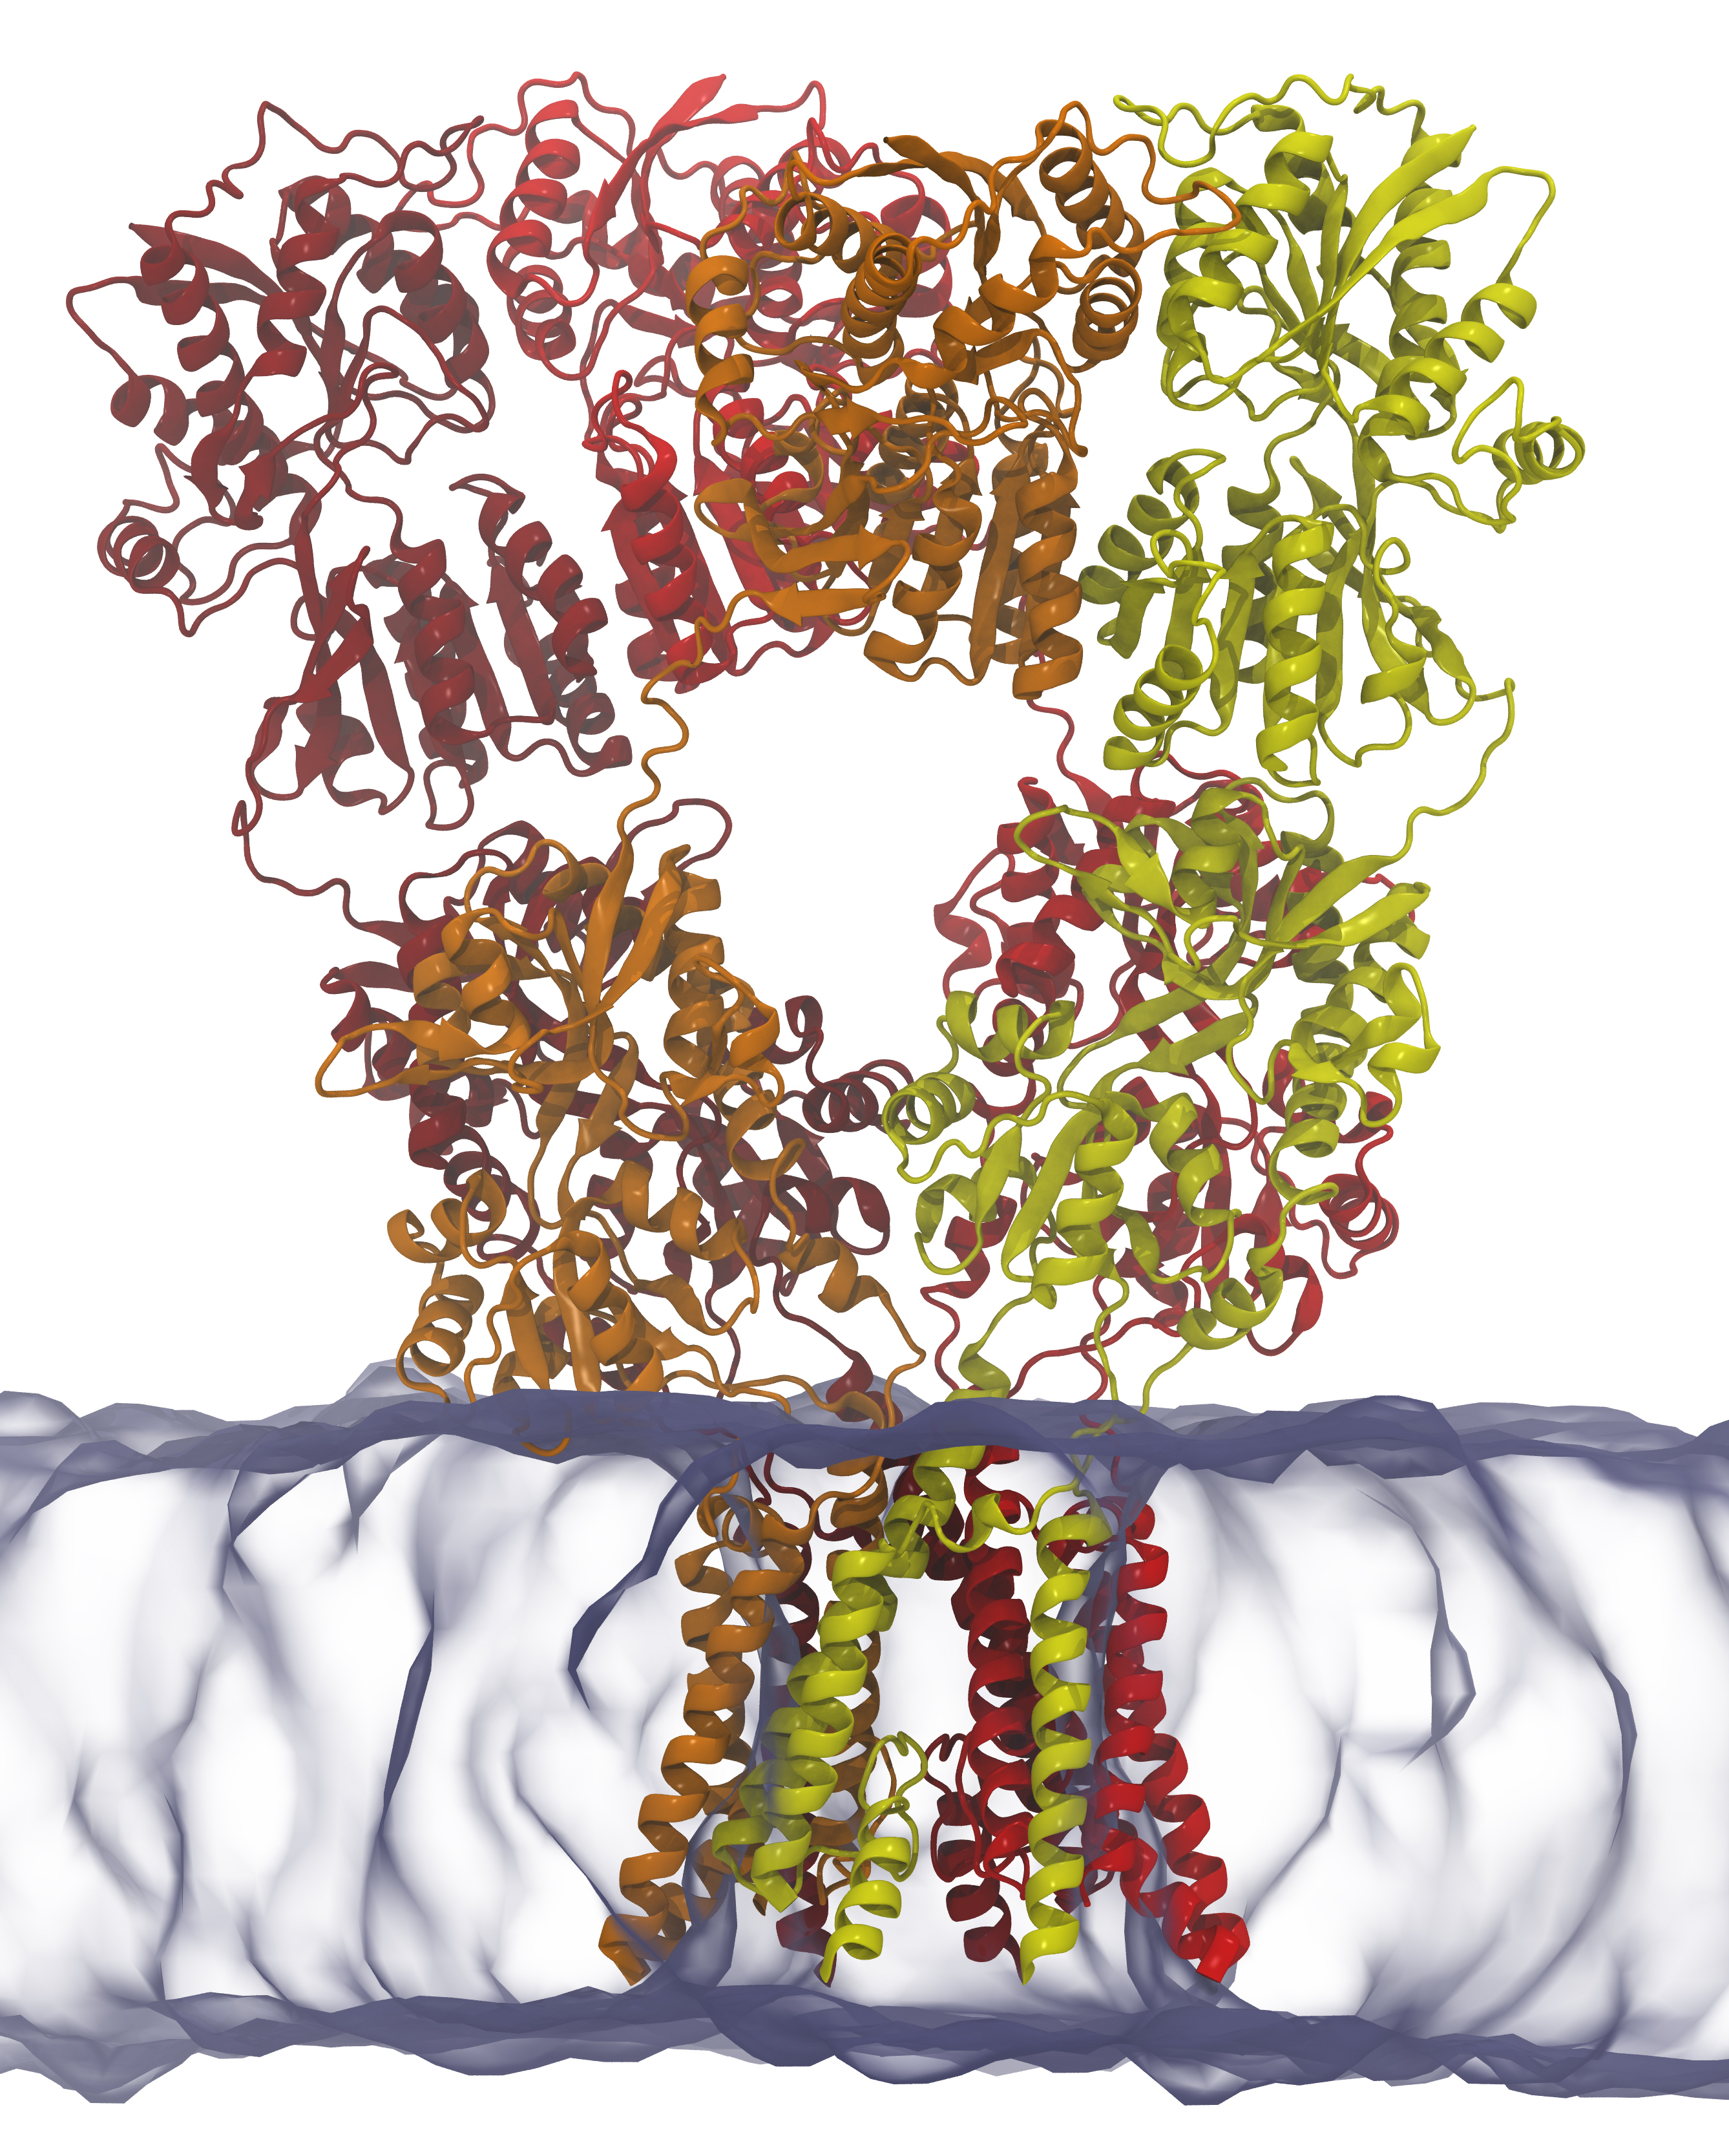
\includegraphics[width=0.4\textwidth]{graphics/glutamate.jpg}\\
  {\small Quelle: \url{http://computation.llnl.gov/glutamate-receptor-molecular-dynamics-simulation} }
\end{frame}

\begin{frame}{Die Programmiersprache C}{Vorlesung \arabic{lecturecounter}}
  \centering
  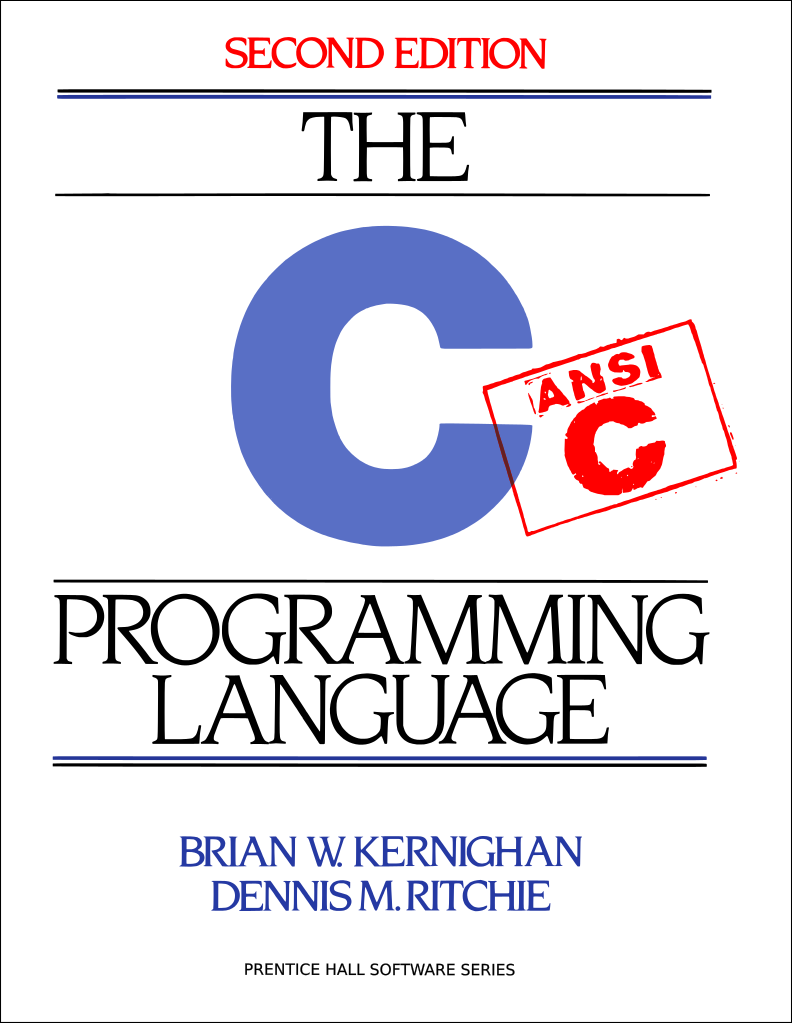
\includegraphics[height=7cm]{graphics/The_C_Programming_Language_cover}
\end{frame}

\begin{frame}{Algorithmus: Einfügensortieren Pseudocode}{Vorlesung \arabic{lecturecounter}}
  \begin{algorithmic}
  \Procedure{insertionsort}{$U,S$}
    \State \textbf{Input:} Lists $U,S$
    \State \textbf{Output:} List $S$
    \For {$i=0$ \textbf{to} \textbf{length}(U)-$1$}
      \State $S_i \gets U_i$
      \State $j \gets i$
      \While {$j > 0$}
        \If{ $S_j < S_{j-1}$}
          \State $t \gets S_j$
          \State $S_j \gets S_{j-1}$
          \State $S_{j-1} \gets t$
          \State $j \gets j-1$
        \Else
          \State \textbf{break}
        \EndIf
      \EndWhile
    \EndFor
  \EndProcedure
\end{algorithmic}

\end{frame}

\begin{frame}[fragile]{Die Struktur eines C-Programms}{Vorlesung \arabic{lecturecounter}}
Das einfache Programm
\begin{lstlisting}
#include <stdio.h>
int main(void){
  printf("Hallo, Welt!\n");
  return 0;
}
\end{lstlisting}
können wir in einer Textdatei \verb|hallo_welt.c| abspeichern und mit dem C-Compiler in ein ausführbares Programm übersetzen
\begin{verbatim}
$ gcc -Wall -Wpedantic -std=c99 -o hallo_welt hallo_welt.c
\end{verbatim}
und es dann ausführen
\begin{verbatim}
$ ./hallo_welt
Hallo, Welt!
$ _
\end{verbatim}
\end{frame}

\begin{frame}[fragile]{Variablen deklarieren und definieren}{Vorlesung \arabic{lecturecounter}}
 Eine Variable wird in C mit:
\begin{lstlisting}
DATENTYP NAME;        // deklariert
NAME = WERT;          // definiert
DATENYP NAME = WERT;  // deklariert und definiert
\end{lstlisting}
 \begin{block}{Blöcke und Sichbarkeitsbereich (\emph{scope})}
 In C werden Programmblöcke mit $\lbrace$ und $\rbrace$ umklammert.
 Ein Block fasst mehrere Ausdrücke (\emph{statements}) zu einem Ausdruck zusammen.
 Eine Variablendeklaration gilt innerhalb eines Blocks und seiner Unterblöcke.
 \end{block}
\begin{lstlisting}
DATENTYP1 VAR1 = WERT1;         // Aeusserster Block
{
  DATENTYP2 VAR2 = WERT2;
  // hier gelten sowohl VAR1 als auch VAR2
  {
    DATENTYP3 VAR3 = WERT3;
    // hier gelten alle drei Variablen
  } // ab hier gilt VAR3 nicht mehr
} // jetzt gilt auch VAR2 nicht mehr
\end{lstlisting}
\end{frame}

\begin{frame}[fragile]{Einrückung und Kommentare}{Vorlesung \arabic{lecturecounter}}
\begin{lstlisting}
DATENTYP1 VAR1 = WERT1;         // Aeusserster Block
{
  DATENTYP2 VAR2 = WERT2;
  // hier gelten sowohl VAR1 als auch VAR2
  {
    DATENTYP3 VAR3 = WERT3;
    // hier gelten alle drei Variablen
  } // ab hier gilt VAR3 nicht mehr
} // jetzt gilt auch VAR2 nicht mehr
\end{lstlisting}
\begin{block}{}
  Ein wichtiger Aspekt, der zur Lesbarkeit eines Quelltextes beiträgt, ist eine konsistente Einrückung der Programmblöcke. Man hätte auch folgendes schreiben können.
\end{block}
\begin{lstlisting}
DATENTYP1 VAR1=WERT1;{DATENTYP2 VAR2=WERT2;{DATENTYP3 VAR3=WERT3;}}
\end{lstlisting}
\begin{block}{}
An nicht-trivialen Stellen des Programmcodes ist es zudem wichtig, dass man Kommentare einfügt, um sich und anderen zu erklären, was da geschieht. 
\end{block}
\end{frame}

\begin{frame}[fragile]{Bedingte Ausführung: \texttt{if / else} Statement}{Vorlesung \arabic{lecturecounter}}
\begin{block}{}
  Das \texttt{if / else} statement erlaubt es, den Programmfluss abhängig vom momentanen Zustand zu steuern.
\end{block}
Input: $x, y, z$
\begin{lstlisting}
if( x > 0 ){
  // x groesser 0
} else if ( x == 0 && y <= 1 ) {
  // x gleich 0 UND y kleiner-gleich 1
  if( (z + 3) == y ){
    // z+3 gleich y
  }
} else if ( x == 0 && y > 1 ) {
  // x gleich 0 UND y groesser 1
} else if ( x < 0 ) {
  // Falls x kleiner 0
}
if( z > 0 || (y % 2 == 0) ){
  // z groesser 0 ODER y gerade
}
\end{lstlisting}
\textbf{Unter welchen Umständen wird keine Anweisung ausgeführt?}
\end{frame}

\begin{frame}[fragile]{Schleifen: \texttt{while} \& \texttt{do-while} (1/2)}{Vorlesung \arabic{lecturecounter}}
\begin{block}{}
  Iterative Verfahren sind ein zentraler Bestandteil vieler Algorithmen.
  Schleifen wiederholen Anweisungen, bis eine gewählte Bedingung erreicht ist.
\end{block}
Die \texttt{while}- und \texttt{do-while}-Schleifen sind die einfachsten Schleifentypen in C und haben folgende Struktur:
\vspace{0.2cm}
\begin{columns}
\column{0.49\textwidth}
\begin{lstlisting}
while( LOGISCHER AUSDRUCK ){
  BEFEHLE
}  
\end{lstlisting}
\begin{enumerate}
  \item[(1)]{ \texttt{AUSDRUCK} auf Wahrheit prüfen }
  \begin{itemize}
    \item[wahr]{ \texttt{BEFEHLE} ausführen }
    \begin{itemize}
      \item[$\drsh$]{Zurück zu (1)}
    \end{itemize}
    \item[unwahr]{ Schleife beenden }
  \end{itemize}
\end{enumerate}

\column{0.49\textwidth}
\begin{lstlisting}
do {
  BEFEHLE
} while( LOGISCHER AUSDRUCK ); 
\end{lstlisting}
\begin{enumerate}
  \item[(0)]{ \texttt{BEFEHLE} ausführen }
  \item[(1)]{ \texttt{AUSDRUCK} auf Wahrheit prüfen }
  \begin{itemize}
    \item[wahr]{ zurück zu (0) }
    \item[unwahr]{ Schleife beenden }
  \end{itemize}
\end{enumerate}

\end{columns}

\end{frame}

\begin{frame}[fragile]{Schleifen: \texttt{while} \texttt{do-while} (2/2)}{Vorlesung \arabic{lecturecounter}}
\begin{block}{}
Wir wollen folgende unendliche Summe berechnen:
\begin{equation*}
  S=\sum_{n=0}^\infty x^n, \quad |x| < 1
\end{equation*}
\end{block}

\begin{lstlisting}
const double x = 0.8;         // x ist eine Konstante
double S = 0.0;               // S_0 = 0
double xn = 1.0;              // x^0 = 1.0
while( xn > 1.0e-12 ){        // Test auf x^n > 1,0 * 10^{-12}
  S = S + xn;
  xn = xn * x;                // x^n
}
\end{lstlisting}
\begin{lstlisting}
do {
  S += xn;
  xn *= x;
while( xn > 1.0e-12 );
\end{lstlisting}

\end{frame}

\begin{frame}[fragile]{Schleifen: \texttt{for} (1/2)}{Vorlesung \arabic{lecturecounter}}
\begin{block}{}
  In C hat eine \texttt{for}-Schleife Kontrollelemente im Schleifenkopf, ideal um mit einer Zählvariable zu arbeiten (aber auch andere Konstrukte sind möglich).
\end{block}
\begin{lstlisting}
for( INITIALISIERUNG; LOGISCHER AUSDRUCK; SCHRITT ){
  BEFEHLE
}
\end{lstlisting}
\begin{enumerate}
  \item[(0)]{\texttt{INITIALISIERUNG} wird ausgeführt}
  \begin{enumerate}
    \item[(1)]{\texttt{LOGISCHER AUSDRUCK} wird auf Wahrheit geprüft}
    \begin{enumerate}
      \item[wahr]{Weiter zu (2)}
      \item[unwahr]{Schleife beenden}
    \end{enumerate}
    \item[(2)]{\texttt{BEFEHLE} werden ausgeführt}
    \item[(3)]{\texttt{SCHRITT} wird ausgeführt}
    \item[$\Rightarrow$]{Zurück zu (1)}
  \end{enumerate}
\end{enumerate}
\end{frame}

\begin{frame}[fragile]{Schleifen: \texttt{for} (2/2)}{Vorlesung \arabic{lecturecounter}}
\begin{block}{}
Die Berechnung der Summe $\sum_{n=0}^{\infty} \, x^n$, könnte man, z.B. so implementieren:
\end{block}
\begin{lstlisting}
const double x = 0.8;
double S = 0.0;
double xn = 1.0;
for( unsigned int n = 0; n < 1000; ++n ){  // max. 1000 Iterationen
  S = S + xn;
  if( xn < 1.0e-12 ){
    break;                        // aus der Schleife ausbrechen
  }                               // selbst wenn n < 1000
  xn = xn * x;
}
\end{lstlisting}

\begin{block}{}
Oder aber auch so:
\end{block}
\begin{lstlisting}
const double x = 0.8;
double S = 0.0;
for( double xn = 1.0; xn > 1.0e-12; xn *= x){
  S += xn;
}
\end{lstlisting}
\end{frame}

\stepcounter{lecturecounter}

\begin{frame}{Fragen zu Vorlesung 1}
  In der letzten Vorlesung:
  \begin{itemize}
    \item{Rechnerarchitektur}
    \item{Dualsystem}
    \item{Fließkommazahlen}
    \item{(sehr knappe) Einführung in Algorithmen und Pseudocode}
    \item{Erstes C-Programm}
    \item{Kompilieren und Ausführen}
    \item{Datentypen}
    \item{Operatoren}
    \item{Kontrollstrukturen}
    \begin{itemize}
      \item{\texttt{if / else if / else}}
      \item{Schleifen}
      \begin{itemize}
        \item{\texttt{do-while}, \texttt{while}}
        \item{\texttt{for}}
      \end{itemize}
    \end{itemize}
  \end{itemize}
  \textbf{Heute:} Biete: mehr Demos. Suche: mehr kritische Fragen, fallen Sie mir ins Wort, bitte! Auch die Tutoren!
\end{frame}

\begin{frame}{Wieso eigentlich C?}{Vorlesung 1 Addendum}
  In den nächsten beiden Tagen wird Ihnen vielleicht klar werden, dass einige Aspekte von C doch komplizierter sind, als man glaubt. Wieso also C nutzen und nicht Python?
  \vspace{0.3cm}
  \begin{itemize}
    \item{C und C++ schaffen einen Spagat zwischen Nähe an der Hardware und einer relativ einfachen Sprachsyntax.}
    \begin{itemize}
      \item{Wissenschaftliche Software muss oft so schnell wie möglich sein.}
      \item{Effiziente Programmierung und gute Compiler machen dies in C und C++ möglich.}
    \end{itemize}
    \vspace{0.4cm}
    \item{In der Wissenschaft gibt es unglaublich viel Software die ursprünglich in C geschrieben wurde oder immer noch geschrieben wird. In Bacheror- Master- oder Doktorarbeiten, werden Sie damit in Kontakt kommen und müssen die ``hässlichen'' Grundlagen ein Mal gesehen haben.}
    \vspace{0.4cm}
    \item{Andere Sprachen machen ``unter der Motorhaube'' nichts anderes als C. Zu verstehen, was genau der Rechner da tun muss, hilft zu verstehen, wieso einige Dinge ineffizient sein könnten.}
  \end{itemize}
\end{frame}

\begin{frame}[fragile]{Textausgabe Mini-Intro}{Vorlesung \arabic{lecturecounter}}
  \begin{block}{\texttt{printf} und die Formatspezifikation}
    \texttt{printf} ist eine Funktion zur \emph{formatierten} Textausgabe in der Konsole.
    Um verschiedene Datentypen auszugeben, muss man Platzhalter nutzen.
  \end{block}
  \begin{center}
  \begin{tabular}{lr}
    \hline
    \texttt{Platzhalter} & Bedeutung \\\hline
    \texttt{\%d}        &  \texttt{int} \\
    \texttt{\%ld}  &  \texttt{long int} \\
    \texttt{\%lld} &  \texttt{long long int} \\
    \texttt{\%ud}  &  \texttt{unsigned int} \\
    \texttt{\%llu} &  \texttt{long long unsigned int} \\
    \texttt{\%f,\%e}   & \texttt{float} \\
    \texttt{\%lf,\%le}  & \texttt{double} \\
    \hline
  \end{tabular}
  \end{center}  
  \begin{block}{}
    $\Rightarrow$ Mal ausprobieren! (\verb|test_printf.c|)
  \end{block}
\end{frame}

\begin{frame}[fragile]{Funktionen}{Vorlesung \arabic{lecturecounter}}
  \begin{block}{}
    C-Programme bestehen im Wesentlichen aus Funktionsdefinitionen und Funktionsaufrufen, sowie eingebauten und eigenen Datentypen. Ein komplexes C-Programm ruft viele Funktionen auf, welche wiederum Funktionen aufrufen.
  \end{block}
  \centering
  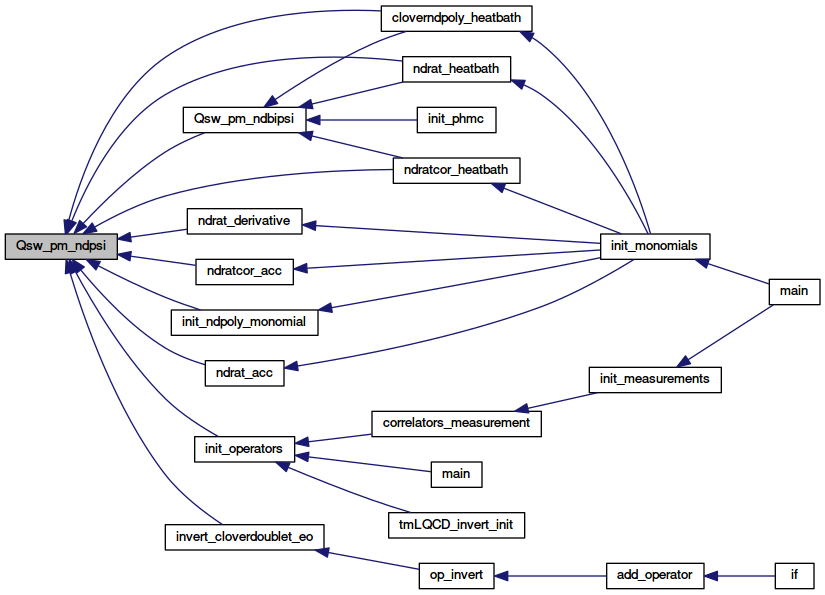
\includegraphics[height=7cm]{graphics/call_graph}
\end{frame}

\begin{frame}[fragile]{Funktionen: Definition}{Vorlesung \arabic{lecturecounter}}
\begin{block}{}
In der letzten Vorlesung hatten wir ein Programm entwickelt um eine Annäherung an die unendliche Summe
\begin{equation*}
  S=\sum_{n=0}^\infty x^n, \quad |x| < 1
\end{equation*}
zu bestimmen.
\end{block}
\begin{lstlisting}
const double x = 0.8;
double S = 0.0;
double xn = 1.0;
for( unsigned int n = 0; n < 1000; ++n ){  // max. 1000 Iterationen
  S = S + xn;
  if( xn < 1.0e-12 ){
    break;                        // aus der Schleife ausbrechen
  }                               // selbst wenn n < 1000
  xn = xn * x;
}
\end{lstlisting}
\textbf{Wir wollen nun mit einer Funktion die Berechnung auslagern und verallgemeinern.} (\verb|sum_xn_funktion.c|)
\end{frame}

\begin{frame}[fragile]{Funktionen: Funktionskopf und Signatur}{Vorlesung \arabic{lecturecounter}}
\begin{block}{}
  Eine Funktion wird dem Compiler bekannt gemacht, indem ihr Name und die Datentypen ihrer Argumente festgelegt werden. $\Rightarrow$ \emph{Funktionsdeklaration}
\end{block}

\begin{lstlisting}
RUECKGABETYP FUNKTIONSNAME( ARGUMENT1_TYP ARG1, ARGUMENT2_TYP ARG2,
                            ARGUMENT3_TYP ARG3 );
\end{lstlisting}
\begin{block}{Signatur}
  Dies nenn man auch die \emph{Signatur} der Funktion.
  {\footnotesize \verb| (FUNKTIONSNAME) ( ARGUMENT1_TYP, ARGUMENT2_TYP, ARGUMENT3_TYP ) | }
\end{block}
\textbf{Korrektur aus der Vorlesung:} Es darf nur eine Funktion mit dem Namen \texttt{FUNKTIONSNAME}.
\end{frame}

\begin{frame}[fragile]{Funktionen: Funktionsaufruf und Rückgabewert}{Vorlesung \arabic{lecturecounter}}
\begin{block}{}
Hat eine Funktion einen Rückgabewert, so kann man diesen beim Aufruf einer Variable zuweisen:
\begin{lstlisting}
double result = teilen( 8.0, 3.2 );  
\end{lstlisting}
\end{block}
\begin{block}{}
Man kann den Rückgabewert aber auch einer anderen Funktion als Argument übergeben:
\begin{lstlisting}
addieren( teilen(8.0, 3.2), 4.5 );
\end{lstlisting}
\begin{itemize}
  \item{Was macht dieser Code?} 
\end{itemize}
\end{block}
\begin{block}{}
Oder aber man ignoriert den Rückgabewert, wie wir es bei \texttt{printf([...])} getan haben (Gesamtzahl der geschriebenen Zeichen).
\end{block}
\end{frame}

\begin{frame}[fragile]{Funktionen: Deklaration und Definition}{Vorlesung \arabic{lecturecounter}}
\begin{block}{}
  Die \emph{Funktionsdeklaration} informiert den Compiler über die Existenz und Signatur einer Funktion
\begin{lstlisting}
double power( const double, const int );
\end{lstlisting}
\end{block}
\begin{block}{}
  Die \emph{Funktionsdefinition} beschreibt erst, wie diese Funktion ihre Aufgabe erfüllt.
\end{block}
Funktionsdeklarationen führen einerseits zu lesbarerem Code, finden aber andererseits Verwendung in der \emph{modularen Programmierung}, die wir in den nächsten Tagen kennenlernen werden.

\textbf{Erstmal ein Beispiel.} (\verb|funktion_deklaration.c|)
\end{frame}

\begin{frame}[fragile]{Funktionen: Rekursion}{Vorlesung \arabic{lecturecounter}}
  \begin{block}{Rekursion}
    Eine Funktion, die sich selbst aufruft, nennt man \emph{rekursiv}. Rekursion kann man oft nutzen, um Aufgaben auf fast magische Art und Weise zu lösen. Leider birgt Rekursion auch viele Gefahren.
  \end{block}
\begin{lstlisting}
TYP rekursion( TYP arg ){
  if( [...] ){ // Ziel erreicht!
    return arg;
  } else {
    return rekursion( arg ); // noch einmal tiefer verschachteln!
  }
}
\end{lstlisting}
   \textbf{Versuchen wir mal, unsere Summe rekursiv auszurechnen!} (\verb|sum_xn_rekursiv.c|)
\end{frame}
 
\begin{frame}[fragile]{\texttt{gdb} und \texttt{valgrind}}
\begin{block}{}
  Nanu, was ist denn da schiefgegangen? Ein Debugger, ist ein Programm, mit dem man Fehler in anderen Programmen versuchen kann nachzuvollziehen.
\end{block}
\begin{block}{Debugging-Symbole mit einbinden und Programm in \texttt{gdb} ausführen}
\begin{verbatim}
$ gcc -Wall -Wpedantic -g -ggdb -std=c99 \
  -o sum_xn_rekursiv_DEBUG sum_xn_rekursiv.c
$ gdb ./sum_xn_rekursiv_DEBUG
GNU gdb (Ubuntu 7.11.1-0ubuntu1~16.04) 7.11.1
(gdb) run
\end{verbatim}
\end{block}

\begin{block}{\texttt{valgrind}}
Ein weiteres nützliches Programm ist \texttt{valgrind}. Es ist eigentlich kein Debugger im eigentlichen Sinne, ist aber spezialisiert darauf, Speicherfehler zu erkennen.
\begin{verbatim}
$ valgrind ./sum_xn_rekursiv_DEBUG
\end{verbatim}
\end{block}
\end{frame}

\begin{frame}[fragile]{Statische Arrays}{Vorlesung \arabic{lecturecounter}}
  \begin{block}{}
    Oft brauchen wir viele Daten des gleichen Datentyps. Diese kann man praktisch in \emph{Arrays} abspeichern.
  \end{block}

\begin{lstlisting}
DATENTYP NAME[ANZAHL];
\end{lstlisting}
Hierbei muss, selbst in C99, \texttt{ANZAHL} fast immer eine numerische Konstante sein!

\begin{lstlisting}
double a[3];  // Array mit 3 double deklarieren

double b[3] = {1.0, 2.3, 9.9};  /* Array mit 3 double deklarieren
                                   und initialisieren */

double c[4] = {4.5, 7.3}; /* Die ersten beiden Elemente mit 
                             4.5 und 7.3 initialisieren,
                             alle anderen werden mit 0.0 
                             initialisiert */
                                   
a[1] = 0.0001; // 0.0001 im zweiten Element von v abspeichern
\end{lstlisting}
\textbf{$\Rightarrow$ Wir möchten nun für unsere Annäherung an die unendliche Summe alle Terme abspeichern und ausgeben!} (\verb|sum_xn_alleterme.c|)
\end{frame}

\begin{frame}[fragile]{Mini-Intro: Texteingabe}{Vorlesung \arabic{lecturecounter}}
\begin{block}{Der Adressoperator \texttt{\&}}
  Für jede Variable, jedes Datentyps, gibt \texttt{\&} die Speicheradresse der Variable zurück. (Um genauer zu sein, ist der Rückgabewert ein Zeiger auf ein Objekt des ensprechenden Datentyps)
\end{block}
\begin{block}{Eingabe mit \texttt{scanf}}
  Die Funktion \texttt{scanf} kann als umgekehrtes \texttt{printf} verstanden werden.
\end{block}
\begin{lstlisting}
int ganzzahl; double dezimalzahl;
scanf("%d %lf",&ganzzahl, &dezimalzahl);
\end{lstlisting}
\textbf{Probieren wir mal, ob wir so unser Summenprogramm weiter verallgemeinern können.} (\verb|test_scanf.c| und \verb|sum_xn_eingabe.c|)
\end{frame}

\begin{frame}[fragile]{Preview: Zeiger auf Daten}{Vorlesung \arabic{lecturecounter}}
\begin{block}{Zeigervariablen}
  Eine Zeigervariable speichert die Adresse einer Variable für einen bestimmten Datenyp.
\end{block}
\begin{block}{Dereferenzierungsoperator \texttt{*}}
  Dieser Operator gibt Zugriff zu den Daten, auf die der Zeiger zeigt.
\end{block}
$\Rightarrow$ \textbf{Tafelbild +} (\texttt{zeiger\_preview.c})
\end{frame}

\stepcounter{lecturecounter}

\begin{frame}[fragile]{Fragen zu Vorlesung 2}{Vorlesung \arabic{lecturecounter}}
  \begin{itemize}
    \item{Platzhalter in \texttt{printf}}
    \item{C-Programme als Funktionssammlungen}
    \item{Funktionen: Kopf, Signatur, Aufruf, Deklaration, Definition, Rückgabewert, Rekursion}
    \item{Debugger Mini-Mini-Intro}
    \item{Statische Arrays}
    \item{Texteingabe mit \texttt{scanf}}
    \item{Preview: Zeiger}
  \end{itemize}
\end{frame}

\begin{frame}[fragile]{Zeiger}{Vorlesung \arabic{lecturecounter}}
  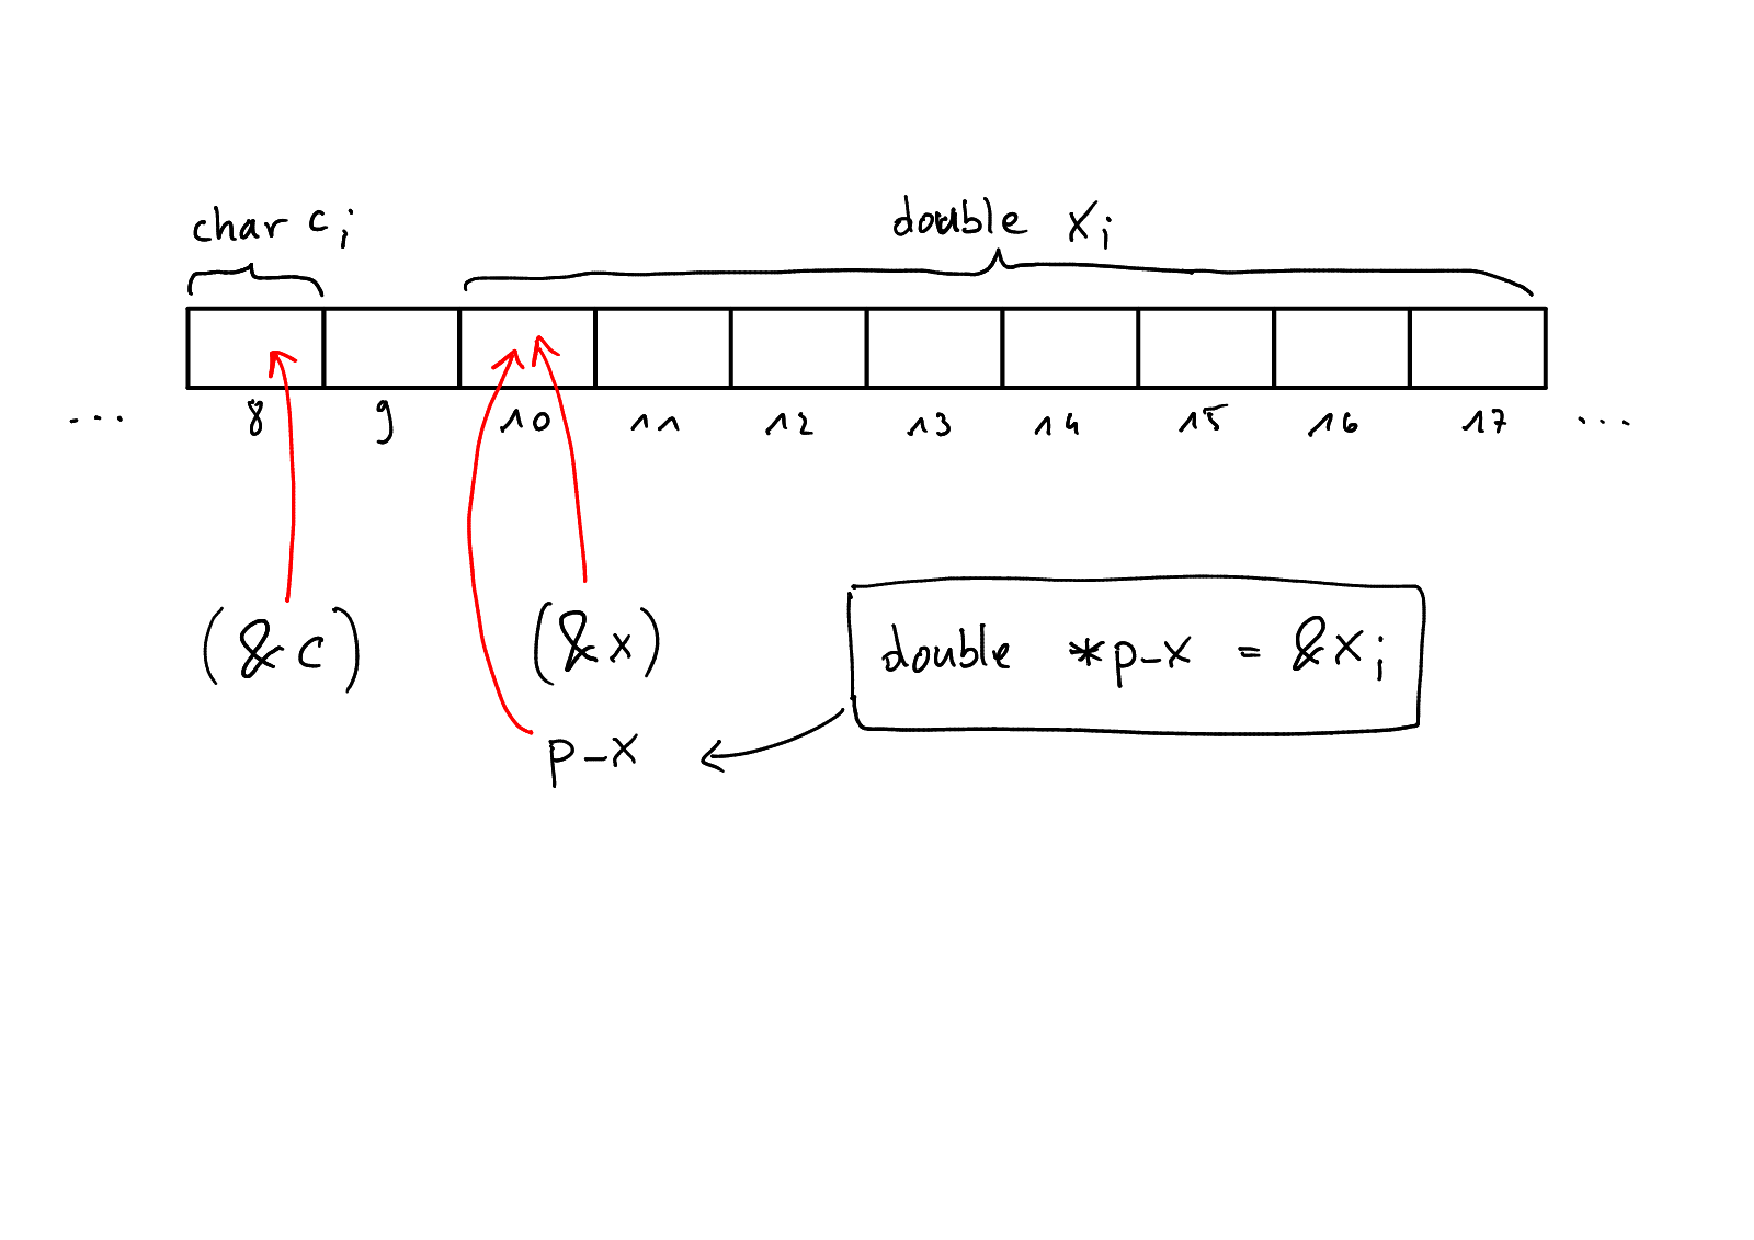
\includegraphics[width=\textwidth,page=1,trim=0 7cm 0 2cm,clip=true]{graphics/c_kurs_tafel}
  \begin{block}{}
    Zeiger sind Datentypen, welche die Adresse einer Variable oder, allgemein, eines Speicherbereichs darstellen.
  \end{block}
  $\Rightarrow$ (\texttt{zeiger\_demo.c}) und Tafelbild
  \begin{block}{}
    Ein \texttt{NULL}-pointer zeigt auf gar nichts. (Strikt gesehen falsch: zeigt auf Adresse '0', diese Adressee darf nicht derefernziert werden! [segmentation fault])
  \end{block}
\end{frame}

\begin{frame}[fragile]{Arrays, Zeiger und einfache Zeigerarithmetik}{Vorlesung \arabic{lecturecounter}}
  \begin{block}{}
    Statische Arrays sind spezielle Speicherbereiche, für die der Compiler einen Standardzeiger setzt. Dieser Zeiger ist der Name des Arrays.
  \end{block}
\begin{lstlisting}
int a[4];   /* 'a' hat Datentyp (int*) und zeigt  
               auf ein Array des Typs (int) */
int *b = a; /* 'b' hat auch den Datentyp (int*) und zeigt jetzt
               auf den gleichen Speicherbereich wie 'a' */
\end{lstlisting}
\begin{block}{}
  Strikt gesehen sind arrays und Zeiger (\emph{pointer}) auf Daten des gleichen Datentyps aber nicht identisch!
\end{block}
 $\Rightarrow$ (\texttt{zeiger\_array\_demo.c}) und Tafelbild

\end{frame}

\begin{frame}[fragile]{Zeichenketten}{Vorlesung \arabic{lecturecounter}}
  \begin{block}{}
    \begin{itemize}
      \item{Die Manipulation von Zeichenketten (auch \emph{strings}) ist in vielen Programmen von zentraler Bedeutung, z.B. um Dateinamen für Ausgabedateien zu setzen.}
      \item{In C werden einfache strings in \texttt{char}-Arrays gespeichert. Da \texttt{char} nur 1B groß ist, stehen einem bloß 255 verschiedene Zeichen zur Verfügung.}
      \item{Strings werden in C \emph{null-terminiert}: Am Ende eines Strings steht ein spezielles Zeichen, welches man auch selbst mit '\textbackslash 0' einfügen kann.}
      \item{Ein C String ist also ein \texttt{char}-Array der Länge $n$ für maximal $n-1$ Zeichen.}
    \end{itemize}
  \end{block}
  \begin{lstlisting}
    // dies ist ein string
    char begruessung[20] = "Hallo, Welt!\n";
    printf("%s", begruessung);
  \end{lstlisting}
  $\Rightarrow$ (\verb|test_strings.c|)
\end{frame}

\begin{frame}[fragile]{Zeichenketten bearbeiten: \texttt{snprintf}}{Vorlesung \arabic{lecturecounter}}
  \begin{block}{}
    \begin{itemize}
      \item{C enthlält viele Funktionen zur Manipulation von Zeichenketten. Fast alle sind unsicher.}
      \item{Es gibt eine Ausnahme: \texttt{snprintf}}
    \end{itemize}
  \end{block}
  (\verb|unsichere_Zeichenketten.c|)  und (\verb|test_snprintf.c|)
\end{frame}

\begin{frame}[fragile]{\emph{Pass-by-reference}: Zeiger an Funktionen übergeben}{Vorlesung \arabic{lecturecounter}}
  \begin{block}{}
    Wie wir gesehen haben, existieren Variablen in C -- sofern es sich nicht um globale Variablen handelt -- nur innerhalb eines Blocks. Aus Effizienzgründen ist es oft aber unratsam, Kopien großer Datenstrukturen hin- und herzuschieben.
  \end{block}
  Wir können aus der Funktion \texttt{inkrement}, nicht einfach so auf \texttt{x} aus der Funktion \texttt{main} zugreifen.
  \begin{lstlisting}
int inkrement(int n){
  x += n; // Fehler: 'inkrement' kennt 'x' nicht!
}  
int main(void){
  int x = 22;
  inkrement(4); // Fehler: 'inkrement' kennt 'x' nicht!
  return 0;
} 
\end{lstlisting}
\vspace{-0.4cm}
  \begin{block}{}
    Mithilfe von Zeigern, können wir Funktionen direkt auf Daten anwenden, welche in einem anderen Block deklariert wurden. (wie bei \texttt{scanf} gemacht)
  \end{block}
  $\Rightarrow$  nächste Folie
\end{frame}

\begin{frame}[fragile]{\emph{Pass-by-reference}: Zeiger an Funktionen übergeben}{Vorlesung \arabic{lecturecounter}}
  \begin{block}{}
    Übergeben wir die Adresse von \texttt{x} an die Funktion, hat diese direkten Zugriff auf die Variable \texttt{x} aus der \texttt{main}-Funktion.
  \end{block}
  \begin{lstlisting}
int inkrement(int *z_x, int n){
  *z_x += n;
}  
int main(void){
  int x = 22;
  inkrement(&x, 4); // x wird von 'inkrement' um 4 inkrementiert
}
\end{lstlisting}
\vspace{-0.4cm}
  \begin{block}{}
    Das können wir auch anhand unserer Summenfunktion zeigen:
  \end{block}
  $\Rightarrow$ (\verb|sum_xn_by_reference.c|)
\end{frame}

\begin{frame}[fragile]{Kommandozeilenargumente}{Vorlesung \arabic{lecturecounter}}
\begin{block}{}
  In unseren Programmen haben wir bisher
\end{block}
\begin{lstlisting}
  int main(void){ [...] } 
\end{lstlisting}
\begin{block}{}
  geschrieben. \texttt{void} bedeutet leer oder auch ungültig. Wir haben damit darauf hingedeutet, dass unsere \texttt{main}-Funktion keine Argumente entgegennimmt.
  \begin{itemize}
    \item{Der \texttt{main}-Funktion werden aber vom Betriebssystem Argumente übergeben: die Kommandozeilenargumente}
  \end{itemize}
\begin{verbatim}
$ ./programm arg0 arg1 arg2
\end{verbatim}
\begin{lstlisting}
int main(int argc, char **argv){
  [...]
}
\end{lstlisting}

\end{block}
$\Rightarrow$ (\texttt{test\_argc.c})
\end{frame}

\begin{frame}[fragile]{Kommandozeilenargumente auslesen}{Vorlesung \arabic{lecturecounter}}
  \begin{block}{}
    \begin{itemize}
      \item{Bei \texttt{**argv} (oder auch \texttt{*argv[]}) handelt es sich um ein Array von Strings (ein Array von \texttt{char}-Arrays).}
      \item{C bietet einige Funktionen, die es erlauben aus Strings andere Datentypen auszulesen.}
      \item{\texttt{sscanf} ist eine mit \texttt{scanf} verwandte Funktion zum Auslesen einzelner Elementer aus formatierten Texten in Variablen}
      \item{Für Kommandozeilenargumente ist es oft praktischer einfachere Funktionen zu nutzen.}
      \begin{itemize}
        \item{\verb|atoi, atof, strtod, strtol, strtoul, strtoull|}
      \end{itemize}
      \item{Aber Vorsicht: \verb|atoi| und \verb|atof| prüfen nicht auf Fehler!}
    \end{itemize}
  \end{block}
  $\Rightarrow$ (\verb|test_read_argv.c|)
\end{frame}

\stepcounter{lecturecounter}

\begin{frame}[fragile]{Fragen zu Vorlesung 3?}{Vorlesung \arabic{lecturecounter}}
  \begin{itemize}
    \item{Zeiger auf Variablen verschiedener Typen}
    \item{Arrays und Zeiger}
    \item{Zeichenketten}
    \item{Zeichenketten bearbeiten}
    \item{Kommandozeilenargumente}
  \end{itemize}
  \vspace{0.5cm}
  Heute gibt es ein physikalisches Beispiel! (yaaay).
\end{frame}

\begin{frame}[fragile]{Rückblick: Zeiger}{Vorlesung \arabic{lecturecounter}}
\begin{block}{}
Die Notation für Zeiger in C ist auf den ersten Blick (meiner Meinung nach) etwas unklar $\rightarrow$ Rückblick
\end{block}
\begin{lstlisting}
  double x; double y; // zwei double Variablen deklarieren
  double arr_y[10]; // und ein double Array mit 10 Elementen
  
  double *z_x, *z_y, w; /* zwei Zeiger auf double ('z_x' und 'z_y')
                         * und ein double ('w') */
   
  z_x = &x; // 'z_x' zeigt jetzt auf 'x'
  z_y = &y; // 'z_y' zeigt jetzt auf 'y'
  
  *z_y = 4.2; // 'z_y' derefernzieren und 'y' auf 4.2 setzen
  
  z_y = arr_y; // Zeiger 'z_y' zeigt jetzt auf 'arr_y'
  
  z_y[0] = 6.2; // erstes Element von 'arr_y' auf 6.2 setzen
  
  z_x = &w; // 'z_x' zeigt jetzt auf 'w'
  
  *z_x = 5.4; // 'w' wird auf 5.4 gesetzt
\end{lstlisting}
  
\end{frame}


\begin{frame}[fragile]{Modulare Programmierung}{Vorlesung \arabic{lecturecounter}}
\includegraphics[width=\textwidth,page=2,trim=0 10cm 0 2cm,clip=true]{graphics/c_kurs_tafel}
\begin{block}{}
  \begin{itemize}
    \item{Themenspezifische Funktionssammlungen können in C in separaten Quelltextdateien stehen und unabhängig voneinander kompiliert werden.}
  \end{itemize}
\begin{enumerate}
  \item{Funktionen in separate Dateien auslagern}
  \item{Einzelne Module kompilieren \\ \texttt{\$ gcc \textcolor{red}{-c} modulX.c} $\rightarrow$ \texttt{modulX.o}}
  \item{Module zu Programm verlinken \\ \texttt{\$ gcc -o programm modul1.o modul2.o}}
\end{enumerate}
\end{block}
\end{frame}

\begin{frame}[fragile]{Modulare Programmierung: Quell- und \emph{Header}-dateien}{Vorlesung \arabic{lecturecounter}}
\small $x$ sei ein Array, welches die $1D$ Position eines Teilchens zur Zeit $t$ enthält. Wir wollen die kinetische Energie berechnen. Die einzelnen \texttt{x[i]} liegen im Abstand von $dt=0.01$.
\begin{columns}[T]
  \column{0.49\textwidth}
    \begin{lstlisting}
#include "AblT.h"
double 
kinEnerg( double *x, 
          double m, 
          unsigned int t ) {
  double v = AblT( x, t );
  return 0.5*m*v*v;
}
    \end{lstlisting}
    \texttt{kinEnerg.c}
    \vspace{0.1cm}
    \begin{lstlisting}
double AblT( double *x, 
             unsigned int t ){
  double dt = 0.01;
  return (x[t+1]-x[t])/dt;
}
    \end{lstlisting}
    \texttt{AblT.c}
  \column{0.49\textwidth}
    \begin{lstlisting}
double kinEnerg( double*, double,
                 unsigned int );
    \end{lstlisting}
    \texttt{kinEnerg.h} \\
    \textcolor{red}{Hier sind die Funktionsdeklarationen.}
    \vspace{2.0cm}
    \begin{lstlisting}
double AblT( double*, 
             unsigned int );
    \end{lstlisting}
    \texttt{AblT.h}  
  \end{columns}
\end{frame}

\begin{frame}[fragile]{Compiler und Linker}{Vorlesung \arabic{lecturecounter}}
  Die Kompilerung und das \emph{Linken} sind unabhängige Schritte bei der Erstellung eines ausführbaren Programms.
\begin{block}{Kompilierung}
  \begin{verbatim}
    # erstellt kinErg.o Objketdatei
$ gcc -c kinEnerg.c

    # erstellt AblT.o   Objektdatei
$ gcc -c AblT.c       

    # erstellt teilchen.o   Objektdatei
$ gcc -c teilchen.c       

    # erstellt ausführbares Programm
$ gcc -o teilchen teilchen.o AblT.o kinEnerg.o 
  \end{verbatim}
\end{block}
$\Rightarrow$ ( \verb|teilchen/kinErg.c teilchen/AblT.c teilchen/teilchen.c|)
\end{frame}

\begin{frame}[fragile]{Modulare Programmierung: Interface und Implementierung}{Vorlesung \arabic{lecturecounter}}
Trennung Interface/Implementierung $\rightarrow$ Implementierung austauschbar!
\begin{columns}[T]
  \column{0.49\textwidth}
    \begin{lstlisting}
#include "AblT.h"
double 
kinEnerg( double *x, 
          double m, 
          unsigned int t ) {
  double v = AblT( x, t );
  return 0.5*m*v*v;
}
    \end{lstlisting}
    \texttt{kinEnerg.c}
    \vspace{0.1cm}
    \begin{lstlisting}
double AblT( double *x, 
             unsigned int t ){
  double dt = 0.01;
  return !@(x[t+1]-x[t-1])/(2*dt)!@;
}
    \end{lstlisting}
    \texttt{AblT\_symmetrisch.c}
  \column{0.49\textwidth}
    \begin{lstlisting}
double kinEnerg( double*, double,
                 unsigned int );
    \end{lstlisting}
    \texttt{kinEnerg.h}
    \vspace{2.4cm}
    \begin{lstlisting}
double AblT( double*, 
             unsigned int );
    \end{lstlisting}
    \texttt{AblT.h}  
  \end{columns}
\end{frame}

\begin{frame}[fragile]{Der C-Präprozessor}{Vorlesung \arabic{lecturecounter}}
\begin{block}{}
  \begin{itemize}
    \item{Wir haben bisher einen Teil des Kompilierprozesses ausgelassen: den Präprozessor.}
    \item{Bevor der Compiler seinen Dienst verrichtet, wird der Quelltext vom Präprozessor bearbeitet.}
  \end{itemize}
\end{block}
\begin{block}{Präprozessorkonstanten und Makros}
  Ein Makro ist ein Stück Code mit einem Namen, welches vom Präprozessor beim Durchlauf in den Quelltext eingefügt wird.
\end{block}
\begin{lstlisting}
// MY_PI wird der Wert des Textes bis zum Ende der Zeile zugewiesen
#define MY_PI 3.1415
\end{lstlisting}
\begin{itemize}
  \item{Schreiben wir jetzt in unserem Programm \verb|MY_PI|, ersetzt der Präprozessor, bevor die Datei kompiliert wird, \verb|MY_PI| durch \texttt{3.1415}}
  \item{Mit den Präprozessorkommandos \verb|#ifdef| und \verb|#ifndef| kann man im Präprozessor die Existenz eines Makros überpüfen}
\end{itemize}
$\Rightarrow$ (\verb|test_makros.c|)
\end{frame}

\begin{frame}[fragile]{Include Guards}{Vorlesung \arabic{lecturecounter}}
\begin{lstlisting}
#include "xyz.h" // "xyz.h" wird eingebunden
\end{lstlisting}
\begin{block}{}
  Wenn eine Header-datei in einem Program mehrfalls eingebunden wird, muss sichergestellt sein, dass die darin enthaltenen Definitionen und Deklaration nur einmal durchgeführt werden! $\rightarrow$ \emph{include guards}
\end{block}
\begin{lstlisting}
#ifndef ABLT_H
#define ABLT_H
double AblT( double*, 
             unsigned int );
#endif // um welches #if[n]def handelt es sich hier? ABLT_H!
\end{lstlisting}
\begin{block}{}
  \begin{enumerate}
    \item{\texttt{AblT.h} wird das erste Mal eingebunden: \verb|ABLT_H| ist nicht definiert.}
    \begin{itemize}
      \item{Definiere \verb|ABLT_H| und deklariere Funktion}
    \end{itemize}
    \item{\texttt{AblT.h} wird zum $(1+n)$-ten Mal eingebunden:}
    \begin{itemize}
      \item{\verb|ABLT_H| ist schon definiert $\rightarrow$ überspringe alles bis zu \texttt{\#endif}} 
    \end{itemize}
  \end{enumerate}
\end{block}
$\Rightarrow$ (\verb|test_include.c|)
\end{frame}

\begin{frame}[fragile]{Zusammengesetzte Datenstrukturen}{Vorlesung \arabic{lecturecounter}}
\begin{block}{}
Konzeptionell ist es oft ratsam, mehrere Variablen zu einem \emph{struct} zusammenzufassen.
Die Position unseres Teilchens könnte in zwei Dimensionen z.B. mit folgender Datenstruktur dargestellt werden:
\end{block}
\begin{lstlisting}[basicstyle=\ttfamily\scriptsize]
struct Position_st {
  double x;
  double y;
};  // Achtung: nach struct Deklaration -> Semikolon

// Variable "teilchen1" vom Typ "struct Position_st"
struct Position_st teilchen1;

teilchen1.x = 1.2;  // Zugriff auf Elemente ueber '.' 
teilchen1.y = 1.3;

struct Position_st teilchen2[1000]; // Array von struct
teilchen2[0].x = 8.3; // Zugriff auf struct-Elemente 
teilchen2[0].y = 4.2; // im Array teilchen2

struct Position_st *z_t; // Zeiger auf "struct Position_st"
z_t = &teilchen1;
z_t->x = 3.3; // Zugriff auf Elemente ueber Zeiger 'z_t' und '->'
\end{lstlisting}
\vspace{-0.1cm}
$\Rightarrow$ (\verb|test_struct.c|)
\end{frame}

\begin{frame}[fragile]{Vorschau: Vorlesung 5}
  \begin{itemize}
    \item{Wünsche?}
    \vspace{0.3cm}
    \item{Mehrdimensionale Arrays}
    \vspace{0.3cm}
    \item{Dynamische Speicherverwaltung}
    \begin{itemize}
      \item{Sicherer Umgang mit Speicher!}
    \end{itemize}
    \vspace{0.3cm}
    \item{Dynamische Arrays}
  \end{itemize}
\end{frame}

\stepcounter{lecturecounter}

\begin{frame}[fragile]{Fragen zu Vorlesung 4?}
  \begin{itemize}
    \item{Modulare Programmierung}
    \item{Trennung: Interface / Implementation }
    \begin{itemize}
      \item[$\Rightarrow$]{\verb|04/test_include.c| enthält jetzt vollen Test für \emph{Include Guards}}
      \item[$\Rightarrow$]{\verb|04/test_makros.c|: Eulersche Zahl in Header-datei mit Include Guards}
    \end{itemize}
    \vspace{0.3cm}
    \item{Zusammengesetzte Datenstrukturen}
    \begin{itemize}
      \item{Addendum: ein \texttt{struct} darf natürlich Elemente verschiedener Datentypen enthalten!}
    \end{itemize}
  \end{itemize}
\end{frame}

\begin{frame}[fragile]{Vervollständigung: Quell- und Headerdateien}{Vorlesung \arabic{lecturecounter}}
  \begin{block}{}
    \small
    \begin{itemize}
      \item{Header- und Quelldateien trennen Interface und Implementierung.}
      \item{Erlaubt iterative Entwicklung: Aufgabe in Algorithmen aufteilen, Interfaces überlegen, Verbindungen aufstellen, Schritt für Schritt implementieren.}
      \item{Benötigte Datenstrukturen können auch in den themengebundenen Headerdateien deklariert werden.}
    \end{itemize}
  \end{block}
\begin{lstlisting}[basicstyle=\ttfamily\scriptsize]
#ifndef ZWEID_MECHANIK_H
#define ZWEID_MECHANIK_H
struct zweiD_vektor_st {
  double x;
  double y;
};
struct zweiD_vektor_st AblT_zweiD( double dt, struct zweiD_vektor_st *pos,
                                   unsigned int t, unsigned int tmax );
#endif // ifndef(ZWEID_MECHANIK_H)
\end{lstlisting}
\vspace{-0.2cm}
\begin{block}{}
  Alternativ könnte man die Deklaration des \verb|struct| auch in eine eigene Header-datei verschieben. (emfohlen)
\end{block}
\end{frame}

\begin{frame}[fragile]{Vervollständigung: Zeiger auf lokale Variablen}{Vorlesung \arabic{lecturecounter}}
  \begin{block}{}
    Die Rückgabe von Zeigern auf lokale Variablen ist nicht zulässig.
  \end{block}
  \begin{lstlisting}
double* test_ptr(void){
  double v = 4.2; // v existiert nur innerhalb des Funktionsblocks!
  return &v; // Compiler warnt, aber kein Fehler!
}
int main(void){
  double *z_v = test_ptr(); // legale Zuweisung, kein Fehler!
  printf("%lf\n", *z_v ); // Segmentation Fault bei Dereferenzierung!
  return 0;
}
  \end{lstlisting}
\end{frame}

\begin{frame}[fragile]{Zeigerarithmetik 1}{Vorlesung \arabic{lecturecounter}}
\begin{block}{}
  Wir hatten die Analogie zwischen Zeigern und Arraynamen schon mehrfach angedeutet. Die folgende Zeigerzuweisungen sind identisch.
\end{block}
\begin{lstlisting}
int k[40]; // int Array mit 40 Elementen
int *z1_k = k;     // Der Arrayname 'k'
int *z2_k = &k[0]; // Die Adresse des ersten Elements von 'k[]'
int *z3_k = z2_k;  // Der Wert des int-Zeigers 'z2_k'
\end{lstlisting}
\begin{block}{}
  Ein Zeiger kann inkrementiert werden. Addition/Subtraktion mit ganzzahligen Konstanten oder Variablen ist ebenso möglich. 
\end{block}
\begin{lstlisting}
z1_k++; z1_k++; // 'z1_k' wird zwei Mal inkrementiert
z2_k = &k[2];   // Adresse des dritten Elements von 'k[]'
int delta_k = 2;
z3_k = z3_k + delta_k; // z3_k um '2' erhoehen
\end{lstlisting}
\begin{block}{}
  Alle drei Zeiger zeigen auf das dritte Element des Arrays \texttt{k}.
\end{block}
$\Rightarrow$ (\verb|test_zeigerarithmetik.c|)
\end{frame}

\begin{frame}[fragile]{Zeigerarithmetik 2}{Vorlesung \arabic{lecturecounter}}
\begin{block}{}
  \texttt{k} ist ein \texttt{int}-Array mit $10$ Elementen, initialisiert mit $\lbrace 42, 55, 17, 34, 421, 17, 11, 9, 117, 629 \rbrace$. Wenn Sie jede Gleichheit verstehen, haben Sie Zeigerarithmetik verstanden.
\end{block}
\centering
\includegraphics[page=3,width=0.8\textwidth,clip=true,trim=0 3cm 0 2cm]{graphics/c_kurs_tafel}
\begin{block}{}
  $\Rightarrow$ \verb|k[n]| ist ein praktisches Kürzel für \verb|*(k+n)|.
\end{block}

\end{frame}

\begin{frame}[fragile]{Dynamische Speicherverwaltung}{Vorlesung \arabic{lecturecounter}}
  \begin{block}{\texttt{malloc} und \texttt{free}}
    \begin{itemize}
      \item{Speicher wird in C mit \texttt{malloc} allokiert und mit \texttt{free} wieder freigegeben.}
      \item{Man sollte immer überprüfen, ob einer Allokation erfolgreich war.}
      \item{Wenn man den Speicher nicht mehr braucht, muss er freigegeben werden, sonst entstehen \emph{memory leaks}.}
    \end{itemize} 
  \end{block}
\begin{lstlisting}
  int n = 300;
  // Platz fuer 300 'double'-Variablen allokieren
  double *x = malloc( sizeof(double) * n );
  if( x == NULL ){
    printf("Speicherallokation fuer 'x' fehlgeschlagen!\n"); 
    exit(32); // Rueckgabewert > 0 bedeutet Fehler
  }
  x[23] = 4.2; x[3] = 2.4; [...] // 'x' verwenden
  free(x); /* Speicher 'x' wird nicht mehr gebraucht
            * -> freigeben */
  /* Programm geht weiter */
\end{lstlisting}
$\Rightarrow$ (\verb|test_malloc.c|)
\end{frame}

\begin{frame}[fragile]{Memory Leaks}{Vorlesung \arabic{lecturecounter}}
\begin{block}{}
  \begin{itemize}
    \item{Wird ein Speicherbereich $a$ einem Zeiger zugewiesen und dann ein weiterer Speicherbereich, $b$, dem gleichen Zeiger zugewiesen, geht die Adresse von $a$ verloren. $\rightarrow$ Speicherleck (memory leak)}
    \item{Der Speicher ist belegt und kann, bis das Programm beendet wird, nicht freigegeben werden.}
    \item{Memory leaks sind Bugs, welche oft erst in den unangenehmsten Situationen auftauchen. Man sollte seine Programme überprüfen wenn möglich.}
  \end{itemize}
\end{block}
\begin{lstlisting}
// Platz fuer 100 'double'-Variablen allokieren
double *x = malloc( sizeof(double) * 100 );
/* x wird einem anderen Speicherbereich zugewiesen
 *   -> Speicherleck */
x = malloc( sizeof(double) * 55 );
free(x); /* free'd nur "malloc( sizeof(double) * 55 )"
          * verloren: "malloc( sizeof(double) * 100 )" */
\end{lstlisting}
$\Rightarrow$ (\verb|memory_leak.c|)
\end{frame}

\begin{frame}[fragile]{Mehrdimensionale Arrays}{Vorlesung \arabic{lecturecounter}}
\begin{block}{Statische Mehrdimensionale Arrays}
  Ein statisches mehrdimensionales Array hat in C eine relativ einleuchtende Notation.
\end{block}
\begin{lstlisting}
double A[3][3];    // 3x3 double Matrix
double B[2][5][7]; // 2x5x7 Tensor mit 3 Indices
\end{lstlisting}
\begin{block}{}
  Ein statisches mehrdimensionales Array ist ein spezielles Objekt in C. Es liegt als ein linearer Datenblock im Speicher.  
\end{block}
\centering
\includegraphics[page=4,width=0.8\textwidth,clip=true,trim=0 12cm 0 2cm]{graphics/c_kurs_tafel}
\begin{block}{}
  Dynamische mehrdimensionale Arrays werden genauso angelegt, um den Zugriff effizient zu machen.
\end{block}
\end{frame}

\begin{frame}[fragile]{Linearisierung Mehrdimensionaler Arrays}{Vorlesung \arabic{lecturecounter}}
\begin{block}{}
  Wir wollen eine $N \times N$ Matrix linear im Speicher ablegen, wie verfahren wir?
\end{block}
\begin{lstlisting}
int N = 42;
double *A = malloc( N*N*sizeof(double) ); // 42^2 doubles
\end{lstlisting}
Der Index \texttt{i} für den Zugriff auf $A_{zs}$, ergibt sich aus der Formel:
\begin{equation*}
  i = s + N \cdot z
\end{equation*}
Für ein Objekt mit $3$ Indizes, $T_{i_0 i_1 i_2}$ der Größe $N_0 \times N_1 \times N_2$, ergibt sich:
\begin{align*}
  i = & i_2 + N_2 \cdot ( i_1 + ( N_1 \cdot i_0 ) ) \\
    = & i_2 + N_2 \cdot i_1 + N_2 \cdot N_1 \cdot i_0 \, ,
\end{align*}
wobei $i_0 \in [ 0, N_0-1 ], i_1 \in [ 0, N_1-1 ], i_2 \in [ 0, N_2-1 ] \Rightarrow i \in [ 0, N_0 \cdot N_1 \cdot N_2 - 1 ]$
\begin{block}{}
  Für unsere Matrix $A$ haben wir also:
\end{block}
\begin{lstlisting}
  A[ 1 + N*2 ] // A_{21}
\end{lstlisting}
\end{frame}

\begin{frame}[fragile]{Dynamische Mehrdimensionale Arrays}{Vorlesung \arabic{lecturecounter}}
\begin{block}{}
  Wir wollen eine $N_0 \times N_1$ Matrix erstellen, aber nicht als statisches Array. Wir wollen es uns aber auch erlauben, darauf mit \texttt{[][]} zuzugreifen. Wie gehen wir vor?
\end{block}
\begin{lstlisting}
unsigned int N_0 = 27;
unsigned int N_1 = 13;
// Speicher fuer N_0*N_1 double-Werte
double *matrix_mem = malloc( N_0*N_1*sizeof(double) );
// Speicher fuer N_0 double-Zeiger
double **Matrix = malloc( N_0*sizeof(double*) );
for( unsigned int z = 0; z < N_0; z++ ){
  Matrix[z] = matrix_mem + N_1*z;
  // oder auch
  // Matrix[z] = &(matrix_mem[N_1*z]);
}
Matrix[2][1] = 2.2;
\end{lstlisting}
$\Rightarrow$ (\verb|lin_multidim_array.c|) und (\verb|dyn_multidim_array.c|)
\end{frame}

\stepcounter{lecturecounter}

\begin{frame}[fragile]{Fragen zu Vorlesung 5?}
  \begin{itemize}
    \item{Zeigerarithmetik}
    \vspace{0.2cm}
    \item{Dynamische Speicherverwaltung}
    \vspace{0.2cm}
    \item{Mehrdimensionale Arrays}
    \vspace{0.2cm}
    \item{Dynamische mehrdimensionale Arrays}
  \end{itemize}
\end{frame}

\begin{frame}{Visualisierung: Dynamischer Matrixspeicher}{Vorlesung \arabic{lecturecounter}}
\begin{block}{}
  Freitag: Vorschlag für alternative Visualisierung der Matrixdatenstruktur aus Vorlesung 5.
\end{block}
\includegraphics[width=0.9\textwidth,page=6,trim=0 4cm 0 2cm,clip=true]{graphics/c_kurs_tafel}
\begin{block}{}
  Vorsicht: Spaltendimension nicht automatisch beschränkt, da es sich bei \texttt{M[z][s]} um ein Alias für \texttt{m + 3*z + s} handelt $\Rightarrow$ \texttt{M[0][3] == M[1][0]}
\end{block}
\end{frame}

\begin{frame}[fragile]{Vervollständigung: Speichermanagement}{Vorlesung \arabic{lecturecounter}}
\begin{lstlisting}
void* memmove(void *dest, void *src, unsigned int n);
\end{lstlisting}
  \begin{block}{}
    Mit \texttt{memmove} werden \texttt{n} Bytes von \texttt{src} nach \texttt{dest} kopiert.
  \end{block}

\begin{lstlisting}
void*  memset(void *dest, int b, unsigned int n);
\end{lstlisting}
  \begin{block}{}
    Mit \texttt{memset} werden \texttt{n} Bytes ab Speicherstelle \verb|dest| auf den Bytewert \verb|b| gesetzt. Oft hat man \verb|b=0|.
  \end{block}
  $\Rightarrow$ (\verb|test_memmove_memset.c|)
\end{frame}

\begin{frame}[fragile]{Vervollständigung: Speichermanagement}{Vorlesung \arabic{lecturecounter}}
\begin{block}{}
  Einen allokierten Speicherbereich der Größe \verb|n_old|, kann man nachträglich mit \verb|realloc| vergrößern oder verkleinern.
\end{block}
\begin{lstlisting}
void* realloc(void *ptr, unsigned int n_new);
\end{lstlisting}
\begin{itemize}
  \item{Der Rückgabewert und \verb|ptr| müssen nicht übereinstimmen!}
  \begin{itemize}
    \item{Schlägt \verb|realloc| fehl, ist der Rückgabewert \verb|NULL|, \verb|ptr| bleibt aber weiterhin allokiert.}
    \item{Wenn nach \verb|ptr+n_old| kein zusammenhängender Speicherberich der Größe \verb|n_new-n_old| verfügbar ist, wird ein neuer Speicherbereich der Größe \verb|n_old| allokiert, die Daten aus \verb|ptr| werden dorthin kopiert, \verb|ptr| freigegeben und ein Zeiger auf den neuen Speicherbereich zurückgegeben.}
  \end{itemize}
  \item{Ist \verb|n_new < n_old|, bleibt der Anfang von \verb|ptr| bis \verb|n_new| unverändert.}
\end{itemize}
\begin{lstlisting}
dt* temp = realloc( ptr, n_new );
if( temp != NULL ){ ptr = temp; }
// ptr verwenden
\end{lstlisting}
  
  $\Rightarrow$ (\verb|test_realloc.c|)
\end{frame}

\begin{frame}[fragile]{Eingabe und Ausgabe: \texttt{fopen}}{Vorlesung \arabic{lecturecounter}}
  \begin{block}{}
    C bietet eine Zahl von Funktionen zur Eingabe und Ausgabe, zunächst muss eine Datei jedoch immer geöffnet werden.
  \end{block}
\begin{lstlisting}
FILE* fopen(char *pfad, char *modus);   
\end{lstlisting}
\begin{block}{}
Modus ist ein \texttt{string}, anhand dessen entschieden wird, welche Dateioperationen durchgeführt werden.
\end{block}
\centering
\small
  \begin{tabular}{lr}
    \hline
    \texttt{modus}  & Bedeutung                           \\\hline
    \verb|"w"|      & (erstellen) (über-)schreiben        \\
    \verb|"r"|      & lesen                               \\
    \verb|"a"|      & erstellen oder hinzufügen           \\
    \verb|"w+"|     & erstellen oder überschreiben + lesen\\
    \verb|"r+"|     & lesen + schreiben (nicht erstellen) \\
    \verb|"a+"|     & wie \verb|"a"| + lesen              \\
    \hline
  \end{tabular}
\begin{block}{}
  Der Rückgabewert von \texttt{fopen} ist bei Erfolg ein \emph{Dateizeiger} auf einen \emph{Stream}, ansonsten ein Nullpointer. $\rightarrow$ auf \texttt{NULL} prüfen!
\end{block}

\end{frame}

\begin{frame}[fragile]{Eingabe und Ausgabe: \texttt{fopen}}{Vorlesung \arabic{lecturecounter}}
\begin{lstlisting}
FILE* ausgabedatei = fopen("/pfad/zu/den/daten/daten.txt", "r");
if( ausgabedetail != NULL ){
  // Datei bereit, ausgelesen zu werden
} else {
  // Datei existiert nicht oder sonstiger Fehler!
}
\end{lstlisting}
\vspace{-0.2cm}
\begin{block}{}
  \footnotesize
  \verb|pfad| kann hierbei absolut sein:
  \begin{itemize}
    \item{UNIX:    \verb|/home/user/pfad/zu/den/daten/daten.txt|}
    \item{Windows: \verb|C:\Eigene Dateien\Dokumente\daten.txt|}
  \end{itemize}
  oder relativ zum Verzeichnis, in dem das Programm ausgeführt wurde:
  \begin{itemize}
    \item{UNIX:    \verb|pfad/zu/den/daten/daten.txt|}
    \item{Window:  \verb|pfad\zu\den\daten\daten.txt|}
  \end{itemize}
  Im zweiten Fall wird der Pfad des momentanen Verzeichnisses vorgestellt.
\end{block}
\begin{block}{}
  \footnotesize
  Erst, nachdem die Datei geschlossen wurde, kann sichergestelllt sein, dass auch alles geschrieben wurde. $\rightarrow$ \texttt{fclose}
\end{block}
$\Rightarrow$ (\verb|test_fopen_fclose.c|)
\end{frame}

\begin{frame}[fragile]{Mit \texttt{fprintf} Textdateien schreiben}{Vorlesung \arabic{lecturecounter}}
\begin{lstlisting}
int fprintf(FILE *fp, char *format, ...);
\end{lstlisting}
\begin{block}{}
  \texttt{fprintf} funktioniert wie \texttt{printf}, mit dem Unterschied, dass ein Dateizeiger übergeben werden muss. Um genau zu steuern, wie die Ausgabe auszusehen hat können die Platzhalter durch Parameter gesteuert werden.
\end{block}
\begin{lstlisting}
  % + - 0 !@BREITE!@ . !@PRAEZISION!@ ll/l/h [d,u,s,c,p,g,e,f]  
\end{lstlisting}
\begin{columns}
\column{0.3\textwidth}
\texttt{format}, \texttt{argument} 
\begin{lstlisting}
%.2f, 2.3453
%5d, 32
%05d, 32
%05d, 999932
%+05d, 32
%-5d, 32, 1
%8.3f, 42.3453
\end{lstlisting}
\column{0.69\textwidth}
Ausgabe
\begin{lstlisting}
2.35
   32
00032
999932
+0032
32   1
  42.345
\end{lstlisting}
\end{columns}
\end{frame}

\begin{frame}[fragile]{Formatierte Textdateien lesen mit \texttt{fscanf}}
\begin{block}{}
  \texttt{(s)scanf} hatten wir kurz erwähnt, als es um Kommandozeilenargumente und das Einlesen von Daten aus der Konsole ging. \verb|fscanf| ist eine ähnliche Funktion für Dateistreams.
\end{block}
\begin{lstlisting}
int fscanf(FILE *stream, const char *format, ...);
\end{lstlisting}
$\Rightarrow$ (\verb|test_fscanf.c|)
\end{frame}

\begin{frame}[fragile]{Mit \texttt{fwrite / fread} Binärdateien schreiben und lesen}{Vorlesung \arabic{lecturecounter}}
\begin{block}{}
  Datenstrukturen in C können direkt blockweise ausgeschrieben und eingelesen werden, solange man einen enstprechenden Speicherbereich allokiert hat.
\end{block}
\begin{lstlisting}
unsigned int fwrite(void* data, unsigned int blockgroesse, unsigned int anzahl, FILE* fp);
unsigned int fread(void* data, unsigned int blockgroesse, unsigned int anzahl, FILE* fp);
\end{lstlisting}
\begin{block}{}
  Um zu prüfen, ob das Ende der Datei erreicht wurde oder ein Fehler aufgetreten ist, werden \texttt{feof} und \texttt{ferror} genutzt.
\end{block}
\begin{lstlisting}
int feof(FILE* fp);
int ferror(FILE* fp);
\end{lstlisting}
$\Rightarrow$ (\verb|test_fwrite_fread.c|) 
\end{frame}

\begin{frame}[fragile]{Den Dateicursor bewegen mit \texttt{fseek}}
\begin{block}{}
  Jede Lese- und Schreiboperation bewegt den Dateicursor des Streams. Um diesen Dateicursor selbst zu bewegen, wird \verb|fseek| genutzt. 
  
  Der Cursor bewegt sich \texttt{offset} Bytes ab Position: \texttt{origin} $\in \lbrace$ \verb|SEEK_SET, SEEK_CUR, SEEK_END| $\rbrace$.
\end{block}
\begin{lstlisting}
int fseek(FILE *stream, long offset, int origin);
\end{lstlisting}
\includegraphics[width=\textwidth,page=5,trim=0 13cm 0 2cm,clip=true]{graphics/c_kurs_tafel}
\begin{block}{}
  Um herauszufinden, wo der Dateicursor sich gerade befindent, kann man \verb|ftell| benutzen.
\end{block}
\begin{lstlisting}
long ftell(FILE *stream);
\end{lstlisting}
$\Rightarrow$ (\verb|test_fseek.c|)
\end{frame}

\stepcounter{lecturecounter}

\begin{frame}[fragile]{Eigene Typen anlegen: \texttt{typedef}}{Vorlesung \arabic{lecturecounter}}
\begin{block}{}
  Hatten in Vorlesung 4 Datenstrukturen kennengelernt. Mit \texttt{typedef} können wir ein Kürzel für einen komplexen Datentyp erstellen.
\end{block}
\begin{lstlisting}
typedef double gleitzahl;
gleitzahl x = 4.2;

typedef struct teilchen_2d_t {
  double x;
  double y;
  double v_x;
  double v_y;
  double m;
  int ladung;
} teilchen_2d_t;

teilchen_2d_t *gasarray = malloc( 10000*sizeof(teilchen_2d_t) );
void zeitschritt_gas( teilchen_2d_t* gas ){ ... }
\end{lstlisting}
\begin{block}{}
  Oft hebt man selbst definierte Datentypen durch ein \texttt{\_t} im Quelltext hervor.
\end{block}
\end{frame}

\begin{frame}[fragile]{Anwendung: Doppelt verkettete Liste}{Vorlesung \arabic{lecturecounter}}
\begin{block}{}
  \textbf{Daten in ein Array einzufügen oder daraus zu entfernen ist teuer.}
  \begin{itemize}
    \item{\textcolor{red}{(einfügen)} Array um $n$ Elemente wachsen lassen (\verb|realloc| ohne Datenverlust aber eventuell mit Kopie)}
    \item{\hspace{1.5cm} Index finden, wo die neuen Element eingefügt, bzw. entfernt werden müssen.}
    \item{\hspace{1.5cm} Existierende Daten ab diesem Index nach vorne \textcolor{red}{(einfügen)} bzw. nach hinten \textcolor{red}{(entfernen)} kopieren.}
    \item{\textcolor{red}{(einfügen)} Daten einfügen.}
    \item{\textcolor{red}{(entfernen)} Array verkleinern.}
  \end{itemize}
\end{block}
\centering
\includegraphics[width=0.9\textwidth,page=7,trim=0 8.2cm 0 7cm,clip=true]{graphics/c_kurs_tafel}
\begin{block}{}
  Mit einer doppelt verketteten Liste, müssen nur jeweils zwei Zeiger gesetzt werden.
\end{block}
\end{frame}

\begin{frame}[fragile]{Doppelt verkettete Liste: Listenelemente}{Vorlesung \arabic{lecturecounter}}
\begin{block}{}
  Als Listenelement dient eine Datenstruktur mit zwei Zeigern und Speicherplatz für die eigentlichen Daten.
\end{block}
\includegraphics[width=0.9\textwidth,page=7,trim=0cm 16cm 0cm 2cm,clip=true]{graphics/c_kurs_tafel}
\begin{columns}
\column{0.5\textwidth}
\texttt{dll.h}
\begin{lstlisting}
#ifndef DLL_H
#define DLL_H
typedef struct dll_node_t {
  struct dll_node_t *next;
  struct dll_node_t *prev;
  double            data;
} dll_node_t;

typedef struct dll_t {
  dll_node_t *first;
  dll_node_t *last;
} dll_t;
\end{lstlisting}
\column{0.5\textwidth}
\begin{lstlisting}
dll_t *dll_create();

void  dll_free(dll_t *list);

dll_node_t* 
dll_insert( dll_t *list, 
            dll_node_t *cursor, 
            double data );

void 
dll_delete( dll_t *list, 
            dll_node_t *delnode);

#endif // ifdef(DLL_H)
\end{lstlisting}
\end{columns}
\end{frame}

\begin{frame}[fragile]{Doppelt verkettete Liste durchlaufen}{Vorlesung \arabic{lecturecounter}}
\begin{block}{}
  In Übung 7 werden Sie eine doppelt verkettete Liste implementieren. Um eine solche Liste zu durchlaufen, kann man folgendes Konstrukt nutzen.
\end{block}
\begin{lstlisting}
dll_t* list = dll_create(); /* erstellen und dann fuellen ... */
/* vorwaerts oder rueckwaerts durchlaufen */
for( dll_node_t *ptr = list->first; ptr != NULL; ptr = ptr->next ){}
for( dll_node_t *ptr = list->last; ptr != NULL; ptr = ptr->prev ){}
\end{lstlisting}
\begin{block}{}
  Es gibt viele weitere Datenstrukturen die vom Prinzip her der ähnlich sind.
  \begin{itemize}
    \item{Einfach verkettete Listen/Ringe: kann nur in eine Richtung durchlaufen werden.}
    \item{Drei- und $n$-fach verkettete Listen: für Baumstrukturen und Graphen}
  \end{itemize}
\end{block}
\end{frame}


\begin{frame}[fragile]{Funktionenpointer}{Vorlesung \arabic{lecturecounter}}
  Ein Ziel ist es, möglichst generisch zu programmieren: eine Funktion soll viele Zwecke erfüllen können.
\begin{block}{Beispiel}
  Wir haben eine Funktion \verb|ableitung_cos|, welche eine Annäherung an die Ableitung des Cosinus berechnet.
\end{block}
\begin{lstlisting}
double ableitung_cos(const double x, const double delta){
  return (cos(x+delta)-cos(x))/delta;
}
\end{lstlisting}
Müssen wir hunderte praktisch identischer Funktionen für alle möglichen Ableitungen implementieren? 
\begin{block}{}
  Ein Funktionenpointer ist ein Zeiger auf eine Funktion, ein Datentyp also, der für die komplette Signatur der Funktion einstehen kann.
\end{block}
\end{frame}

\begin{frame}[fragile]{Funktionenpointer}{Vorlesung \arabic{lecturecounter}}
\begin{lstlisting}[basicstyle=\ttfamily\scriptsize]
unser_struct_t erste_funktion(double, int, int, char, double);
unser_struct_t zweite_funktion(double, int, int, char, double);
unser_struct_t !@(*!@fp!@)!@(double, int, int, char, double);

double void_funktion(void);
double (*void_fp)(void);

unser_struct_t ergebnis, ergebnis2;

fp = erste_funktion;
ergebnis = (*fp)( arg0, arg1, arg2, arg3, arg4 ); // ruft erste_funktion auf

fp = zweite_funktion;
ergebnis2 = (*fp)( arg0, arg1, arg2, arg3, arg4 ); // ruft zweite_funktion auf

fp = void_funktion; // Warnung, aber kein Fehler...

void_fp = void_funktion;
double x = (*void_fp)();
\end{lstlisting}
\begin{block}{}
  Der Funktionenpointer erlaubt es, den Aufruf einer Funktion situationsabhängig zu machen. Achtung: Funktionenpointer sind tükisch und fehleranfällig...
\end{block}
$\Rightarrow$ (\verb|23_void_fpointer.c|)
\end{frame}

\begin{frame}[fragile]{Funktionenpointer: Anwendung}{Vorlesung \arabic{lecturecounter}}
\begin{block}{}
  Wir können jetzt die Ableitungsfunktion verallgemeinern.
\end{block}
\begin{lstlisting}
double ableitung(const double x, const double delta, double (*fp)(double) ){
  return ((*fp)(x+delta)-(*fp)(x))/delta;
}

double abl_wert = ableitung( 1.2, 0.0001, cos );
\end{lstlisting}
\begin{block}{}
  Funktionenpointer können auch auf Gleichheit geprüft werden. Insbesondere könnte man überprüfen, ob ein Funktionspointer auf eine bestimmte Funktion zeigt.
\end{block}
\begin{lstlisting}
double ableitung(const double x, const double epsilon, 
                 double (*fp)(double) ){
  if( fp == tan ){
    /* ohje, das wird schwierig... */
  }
  return ((*fp)(x+epsilon)-(*fp)(x))/epsilon;
}
\end{lstlisting}
\end{frame}

\begin{frame}[fragile]{Komplexe Zahlen}{Vorlesung \arabic{lecturecounter}}
\begin{block}{}
  Seit C99 gibt es in C einen Datentypen für komplexe Zahlen. Es gibt davon mehrere Ausführungen mit unterschiedlicher Fließkommagenauigkeit.
\end{block}
\begin{lstlisting}
#include <complex.h>
double _Complex z = 3.0 + 2.1*I;
float  _Complex w = 4.2 + 4.5*I;
\end{lstlisting}
\begin{block}{}
Das Symbol \texttt{I} entspricht hier $\sqrt{-1}$.  
\end{block}
\begin{lstlisting}
double _Complex x = z * w;  
\end{lstlisting}
\begin{block}{}
  Arithmetische Operationen sind auf dem \texttt{\_Complex} Datentyp wie gewohnt definiert.
\end{block}
\end{frame}

\begin{frame}[fragile]{Komplexe Zahlen}{Vorlesung \arabic{lecturecounter}}
\begin{block}{}
  Zugriff auf Real- und Imaginärteil sowie Betrag und Argument erfolgen über die Funktionen:
\end{block}
\begin{lstlisting}
double creal(const _Complex double); // Realteil
double cimag(const _Complex double); // Imaginaerteil
double cabs(const _Complex double); // Betrag
double carg(const _Complex double); // Argument (Bogenmass)
_Complex double conj(const _Complex double); // Konjugierte
\end{lstlisting}
\begin{block}{}
Ausgabe mit \texttt{[s,f]printf} erfolgt also in zwei Teilen:
\end{block}
\begin{lstlisting}
printf("z = %lf + i %lf\n", creal(z), cimag(z));
\end{lstlisting}
\begin{block}{}
  Weitere Funktionen: 
  \begin{itemize}
    \item{\verb|cexp, clog, csqrt, cpow|}
    \item{\verb|csin, ccos, ctan, casin, cacos, catan|}
    \item{\verb|csinh, ccosh, ctanh, casinh, cacosh, catanh|}
  \end{itemize}
\end{block}
\end{frame}

\stepcounter{lecturecounter}

\begin{frame}[fragile]{Uebungen Mittwoch und Donnerstag}{Vorlesung \arabic{lecturecounter}}
\begin{block}{}
  Morgen, Donnerstag den 13.04, keine Vorlesung sondern Übung. Es wird um die Implementation einer größeren Datenstruktur und eines Sortieralgorithmus gehen, anhand dessen die Eigenschaften dieser Datenstruktur dargestellt werden.
\end{block}
\includegraphics[width=\textwidth,page=8,trim=0 9cm 0 2cm,clip=true]{graphics/c_kurs_tafel}
\begin{block}{}
  Heute: Verwendung externer Bibliotheken, kompilieren mithilfe von \verb|make|, vertrauenswürdige Zeitmessung, gute Zufallszahlen, Abbruchbedingungen.
\end{block}
\end{frame}

\begin{frame}[fragile]{Externe Bibliotheken}{Vorlesung \arabic{lecturecounter}}
\begin{block}{Einbinden und Kompilieren}
  Eine ``externe'' Bibliothek hatten wir schon kurz kennengelernt und genutzt: \verb|math.h|. 
\end{block}
\begin{lstlisting}
#include <math.h>
\end{lstlisting}
\begin{block}{}
Um auf die Funktionen aus der Bibliothek dann auch Zugriff zu erhalten, muss diese auch eingelinkt werden:
\begin{verbatim}
gcc -o programm main.o modul1.o modul2.o -lm 
\end{verbatim}
Das Kürzel \verb|-l| bedeutet: suche in den Systembibliothekspfaden nach einer Bibliothek Namens \verb|m|. Oftmals müssen auch weitere Bibliothekspfade angegeben werden. Dies wird mit \verb|-Lpfad| erreicht, wobei \verb|pfad| durch den den zu verwendenden Pfad ersetzt wird.
\end{block}
\end{frame}

\begin{frame}[fragile]{Zufallszahlen mit GSL}{Vorlesung \arabic{lecturecounter}}
\begin{block}{}
  In Übung 5 wurde ein Pseudozufallszahlengenerator entwickelt und mit Conway's Game of Life getestet. Den Standardgenerator in C sollte man nicht benutzen. Gute Alternativen finden sich in der GNU Scientific Library (GSL).
\end{block}
\begin{lstlisting}[basicstyle=\ttfamily\scriptsize]
#include <stdio.h>
#include <gsl/gsl_rng.h>
int main (void) {
  const gsl_rng_type * generator_type;
  gsl_rng * r;
  gsl_rng_env_setup();
  generator_type = gsl_rng_ranlxd2;
  r = gsl_rng_alloc(generator_type);
  double u = gsl_rng_uniform(r);
  for(int i = 0; i < n; i++) {
      u = gsl_rng_uniform (r);
      printf ("%.5f\n", u);
  }
  gsl_rng_free(r);
  return 0;
}
\end{lstlisting}
Probieren wir gleich, erstmal sollten wir jedoch ein wenig mehr über Kompilierung lernen.
\end{frame}

\begin{frame}[fragile]{Einfache Makefiles}{Vorlesung \arabic{lecturecounter}}
\begin{block}{}
Ein Makefile ist eine Datei in der die Regeln zum Kompilieren eines Programms beschrieben sind. Die genaue Struktur ist dabei relativ offen, da es sich nur um Regeln zur Erstellung von Dateien und deren Abhängigkeiten handelt.
\end{block}
\begin{lstlisting}[basicstyle=\ttfamily\scriptsize]
!@regel:!@ abhaenkigkeit1 abhaengigkeit2 abhaengikeit3
        kommando1
        kommando2
\end{lstlisting}
\begin{itemize}
  \item{Um \verb|regel| (auch target oder Ziel genannt) zu erstellen, überprüft \verb|make| zunächst ob die Abhängigkeiten existieren. Wenn ja, werden die Kommandos ausgeführt. Wenn nicht, wird versucht Regeln zu finden um die Abhängigkeiten zu erstellen.}
  \item{Ist eine Abhängigkeit, oder eine Abhängigkeit einer Abhängigkeit (z.B. der C-Quelltext zu einem Modul) neuer als das momentan vorhandene Ziel, wird das Ziel erneut kompiliert.}
  \item{Target und Abhängigkeiten sind durch einen Doppelpunkt getrennt. In der nächsten Zeile ist ein Tabulator (wichtig, keine einfachen Leerzeichen!)}
\end{itemize}
\end{frame}

\begin{frame}[fragile]{Makefiles: Beispiel 1}{Vorlesung \arabic{lecturecounter}}
\begin{block}{}
  Variablen werden in Makefiles mit dem Dollarzeichen referenziert. Es gibt einige spezielle Variablen, aber man kann auch welche selbst definieren.
\end{block}
\begin{lstlisting}[basicstyle=\ttfamily\scriptsize]
test_printf: test_printf.c
        gcc -std=c99 -Wall -Wpedantic -o !@$@ $<!@
\end{lstlisting}
\begin{block}{}
\begin{itemize}
  \item{\verb|$@| ist ein Platzahlter für den Namen des Targets. (hier \verb|test_printf|)}
  \item{\verb|$<| steht für die erste Abhängigkeit von links. (hier \verb|test_printf.c|)}
\end{itemize}
Kompiliert wird jetzt mit:
\begin{verbatim}
 $ make
\end{verbatim}
\verb|make| wird das kommando
\begin{verbatim}
gcc -std=c99 -Wall -Wpedantic -o test_printf test_printf.c
\end{verbatim}
aufrufen und die ausführbare Datei \verb|test_printf| wird dadurch erzeugt werden.
\end{block}
\end{frame}

\begin{frame}[fragile]{Makefiles: Beispiel 2}{Vorlesung \arabic{lecturecounter}}
\begin{lstlisting}[basicstyle=\ttfamily\scriptsize]
# Regeln fuer main-Objektdateien
programm1.o: programm1.c modul1.h modul2.h
        gcc -std=c99 -Wall -Wpedantic -c $<

programm2.o: programm2.c modul2.h modul3.h
        gcc -std=c99 -Wall -Wpedantic -c $<        

# Regel fuer die Module
%.o : %.c %.h    
         gcc -std=c99 -Wall -Wpedantic -c $<

programm1: programm1.o modul1.o modul2.o
        gcc -std=c99 -Wall -Wpedantic -o $@ !@$^!@

programm2: programm2.o modul2.o modul3.o
        gcc -std=c99 -Wall -Wpedantic -o $@ !@$^!@        
\end{lstlisting}
\begin{block}{}
\verb|$^| ist ein Kürzel für alle Abhängigkeiten. Das Kommando:
\begin{verbatim}
 $ make programm1
\end{verbatim}
wird erst \verb|modul1.o, modul2.o| und \verb|programm1.o| kompilieren und dann den Linker aufrufen.
\end{block}
\end{frame}

\begin{frame}[fragile]{Makefiles: Beispiel 3}{Vorlesung \arabic{lecturecounter}}
\begin{block}{}
  Für die ganzen Beispielprogramme, die in der Regel aus einer Datei bestehen, habe ich folgendes Makefile genutzt.
\end{block}
\begin{lstlisting}[basicstyle=\ttfamily\scriptsize]
SOURCES := $(wildcard *.c)                                                                                                                                  

!@all: $(basename $(SOURCES)) !@

$(basename $(SOURCES)): % : %.c Makefile
        gcc -g -ggdb -Wall -Wpedantic -std=c99 -o $@  $<

.PHONY: clean
clean:
        rm $(basename $(SOURCES))
\end{lstlisting}
\begin{itemize}
  \item{\verb|make| führt, wenn es ohne Kommandozeilenargumente aufgerufen wird, die erste Regel aus. Das ist hier \verb|all|. Es werden also alle Programme erzeugt, deren C-Dateien sich in der Variable \verb|$(SOURCES)| wiederfinden.}
\end{itemize}
$\Rightarrow$ (\verb|makefiles/beispiel3|)
\end{frame}

\begin{frame}[fragile]{Makefiles: Einfache Substitutionen}{Vorlesung \arabic{lecturecounter}}
\begin{lstlisting}[basicstyle=\ttfamily\scriptsize]
SOURCES := !@$(wildcard *.c)!@                                                                                                                                   

all: !@$(basename $(SOURCES))!@

!@$(basename $(SOURCES))!@: % : %.c Makefile
        gcc -g -ggdb -Wall -Wpedantic -std=c99 -o $@ $<

.PHONY: clean
clean:
        rm !@$(basename $(SOURCES))!@
\end{lstlisting}
\begin{block}{}
\begin{itemize}
  \item{Mit ``\verb|VARIABELNAME :=|'' werden eigene Variablen definiert.}
  \item{\verb|$(wildcard *.c)| sucht im momentanen Verzeichnis nach allen C-Dateien. Die Dateinamen werden in der Variable \verb|$(SOURCES)| abgelegt.}
  \item{\verb|$(basename $(SOURCES))| entfernt alle Dateiendungen der Dateinamen in der Variable \verb|$(SOURCES)|, hier \verb|.c|}
\end{itemize}
\end{block}
\begin{verbatim}
$(basename programm1.c programm2.c) -> programm1 programm2
\end{verbatim}
\end{frame}

\begin{frame}[fragile]{Makefiles: Das Prozentzeichen}{Vorlesung \arabic{lecturecounter}}
Das Prozentzeichen erlaubt es, Regeln zu automatisieren oder zu verketten.
\begin{block}{}
\begin{lstlisting}[basicstyle=\ttfamily\scriptsize]
!@%!@.o : !@%!@.c !@%!@.h
         gcc -std=c99 -Wall -Wpedantic -c $<
\end{lstlisting}
Für jede Datei des Typs ``\verb|name.o|'' wird eine Abhängigkeit von \verb|name.c| und \verb|name.h| aufgestellt. \verb|name.o| wird dann mit der Regel
\begin{verbatim}
gcc -std=c99 -Wall -Wpedantic -c $<
\end{verbatim}
kompiliert.
\end{block}
\begin{block}{}
\begin{lstlisting}
$(basename $(SOURCES)): !@%!@ : !@%!@.c Makefile
        gcc -g -ggdb -Wall -Wpedantic -std=c99 -o $@ $<
\end{lstlisting}
\begin{itemize}
  \item{Für jedes Objekt in \verb|$(basename $(SOURCES))| wird eine neue Regel erstellt (erstes \%)}
  \item{Für diese neuen Regeln werden Abhängigkeiten der Form \verb|name.c| erstellt und das Kompilierkommando entsprechend ausgeführt.}
\end{itemize}
\end{block}
\end{frame}

\begin{frame}[fragile]{Makefiles: \emph{phony} targets und aufräumen}{Vorlesung \arabic{lecturecounter}}
\begin{lstlisting}[basicstyle=\ttfamily\scriptsize]
!@.PHONY: clean!@
!@clean:!@
        rm $(basename $(SOURCES))
\end{lstlisting}
\begin{block}{}
  \begin{itemize}
    \item{Ein \emph{phony} target kann immer ausgeführt werden, es wird nicht überprüft ob die Datei \texttt{clean} schon existiert.}
    \item{Es ist konventionell, ein solches target mit dem Namen \verb|clean| zu haben, welches alle generierten Dateien aufräumt.}
  \end{itemize}
\end{block}
\begin{block}{}
  Um ein komplexeres Projekt aus mehreren Modulen mit Einbindung von Bilbiotheken und, unter Umständen, mehreren ausführbaren Programmen zu kompilieren, kann uns dieses Beispiel dienen.
\end{block}
$\Rightarrow$ nächste Folie
\end{frame}

\begin{frame}[fragile]{Makefiles: Beispiel 4}{Vorlesung \arabic{lecturecounter}}
\begin{lstlisting}[basicstyle=\ttfamily\tiny]
CC=gcc -std=c99 -Wall -Wpedantic
LD=gcc -std=c99 -Wall -Wpedantic
SOURCES := $(wildcard *.c)
HEADERS := $(wildcard *.h)
MODULES := $(patsubst %.c, %.o, $(SOURCES))
PROGRAMS := teilchen
MODULES := $(filter-out $(addsuffix .o, $(PROGRAMS)), $(MODULES))
LIBS := -lm -lgsl -lgslcblas

all: $(PROGRAMS)

$(addsuffix .o, $(PROGRAMS)): % : $(addsuffix .c, $(PROGRAMS)) $(HEADERS) Makefile
        $(CC) -c $(patsubst %.o, %.c, $@)

%.o: %.c %.h Makefile
        $(CC) -c $<

$(PROGRAMS): % : %.o $(MODULES) Makefile
        $(LD) -o $@ $< $(MODULES) $(LIBS)

.PHONY: clean
clean:
        rm -f $(MODULES) $(PROGRAMS) $(addsuffix .o, $(PROGRAMS))
\end{lstlisting}
$\Rightarrow$ (\verb|makefiles/beispiel4|) hat ausführliche Kommentare, die jede Zeile nochmal erläutern.
\end{frame}

\begin{frame}[fragile]{Zuverlässige Zeitmessung mit \texttt{gettimeofday}}{Vorlesung \arabic{lecturecounter}}
\begin{block}{}
Zeitmessung mit \verb|clock()| ist sehr unzuverlässig. \verb|gettimeofday| wird nicht von anderen Programmen beinflusst und hat eine Präzision von $\mu s$.
\end{block}
\begin{lstlisting}
#include <sys/time.h>
struct timeval anfang, ende;
gettimeofday(&anfang, NULL);
/* Zeit vergeht durch schwierige Rechnungen */
gettimeofday(&ende, NULL);
double sec = (double)(ende.tv_sec-anfang.tv_sec);
double usec = (double)(ende.tv_usec-anfang.tv_usec);
printf("Es sind %lf Sekunden vergangen\n", sec+1.0e-6*usec);
\end{lstlisting}
$\Rightarrow$ (\verb|test_gettimeofday.c|)
\begin{block}{}
  Das \verb|struct timeval| ist wie folgt definiert:
\end{block}
\begin{lstlisting}
struct timeval {
  time_t      tv_sec;     /* seconds */
  suseconds_t tv_usec;    /* microseconds */
};
\end{lstlisting}
\end{frame}

\begin{frame}[fragile]{Abbruchbedingungen mit \emph{assertions}}{Vorlesung \arabic{lecturecounter}}
\begin{block}{}
  \begin{itemize}
    \item{Assertions (Zusicherungen, Sicherstellungen) sind ein Konstrukt, welches es erlaubt, gut lesbare Abbruchkriterien für Ausnahmesituationen zu definieren.} 
    \item{Wenn eine Bedingung nicht gegeben ist, an dieser Stelle im Code aber auf jeden Fall gegeben sein sollte (nicht-\veb|NULL| Argumente in einer Funktion, z.B.), kann man \verb|assert| nutzen, um das Programm dort abzubrechen.}
  \end{itemize}
\end{block}
\begin{lstlisting}
#include <assert.h>
int func(FILE* fp){
  assert( fp != NULL );
  /* ... */
  return 0;
}
int main(void){
  FILE* fp = fopen("gibtbesnicht.txt","r");
  func(fp);
}  
\end{lstlisting}
$\Rightarrow$ (\verb|test_assert.c|)
\end{frame}

\begin{frame}[fragile]{}{Vorlesung \arabic{lecturecounter}}

\begin{minipage}{\textwidth}
  \centering
  \Huge That's all folks!
\end{minipage}
\end{frame}

\end{document}
